%%%%%%%%%%%%%%%%%%%%%%%%%%%%%%%%%%%%%%%%%%%%%%%%%%%%%%%%%%%
% --------------------------------------------------------
% Tau
% LaTeX Template
% Version 2.4.4 (28/02/2025)
%
% Author: 
% Guillermo Jimenez (memo.notess1@gmail.com)
% 
% License:
% Creative Commons CC BY 4.0
% --------------------------------------------------------
%%%%%%%%%%%%%%%%%%%%%%%%%%%%%%%%%%%%%%%%%%%%%%%%%%%%%%%%%%%

\documentclass[9pt,a4paper,twocolumn,twoside]{tau-class/tau}
\usepackage[english]{babel}
% \usepackage{amssymb}
\usepackage{pifont}% http://ctan.org/pkg/pifont
\newcommand{\cmark}{\ding{51}}%
\newcommand{\xmark}{\ding{55}}%

% Bibliography setup
\usepackage[backend=biber,style=ieee]{biblatex}
\addbibresource{references.bib}

%% Spanish babel recomendation
% \usepackage[spanish,es-nodecimaldot,es-noindentfirst]{babel} 

%% Draft watermark
% \usepackage{draftwatermark}

%----------------------------------------------------------
% TITLE
%----------------------------------------------------------

\journalname{Lab Report}
\title{COP290: Rust Lab Report}

%----------------------------------------------------------
% AUTHORS, AFFILIATIONS AND PROFESSOR
%----------------------------------------------------------

\author[a]{Vani Gupta (2023CS10126)}
\author[a]{Arnav Panjla (2023EE10978)}
\author[a]{Basil Labib (2021TT11175)}

%----------------------------------------------------------

\affil[a]{Indian Institute of Technology, Delhi}

\professor{Professor Abhilash Jindal, COP290 TAs}

%----------------------------------------------------------
% FOOTER INFORMATION
%----------------------------------------------------------

\institution{Indian Institute of Technology, Delhi}
\footinfo{\LaTeX\ Lab Report}
\theday{April 24, 2025}
\leadauthor{Gupta et al.}
\course{Creative Commons CC BY 4.0}

%----------------------------------------------------------
% ABSTRACT AND KEYWORDS
%----------------------------------------------------------

\begin{abstract}    
    We added three extensions to the base Rust TUI spreadsheet program, 1) extended functionality such as undo/redo, autofill, etc. to TUI 2) web application to ease usage 3) multi-user, state-consistent CRDT-based WebSocket spreadsheet programme. 
    We will discuss our design decisions, the system architecture for each extension, and the challenges and learnings from this project in this report.
\end{abstract}

%----------------------------------------------------------

\keywords{lab report, rust, spreadsheet, CRDT, webapp, WebSocket}

%----------------------------------------------------------

\begin{document}
		
    \maketitle 
    \thispagestyle{firststyle} 
    \tauabstract 
    % \tableofcontents
    % \linenumbers 
    
%----------------------------------------------------------

\section{Introduction}

    \taustart{W}e proposed a decentralised, state-consistent spreadsheet program. In order to design and build such a complex system, we decomposed it into three checkpoints. We were able to achieve two out of these three checkpoints and one additional checkpoint not included in our proposal. 

    \begin{itemize}
        \item \cmark Browser-based GUI app using client-server architecture
        \item \cmark Centralised state-consistent real-time GUI app using WebSockets and CRDTs
        \item \xmark Decentralised state-consistent real-time GUI app using WebSockets and CRDTs
    \end{itemize}

    In addition, we also extended the base TUI which was not included in our initial proposal.

    \begin{itemize}
        \item \cmark Added undo/redo up to 5 previous steps
        \item \cmark Predict cell values and autofill ranges
        \item \cmark Support for non-integer datatypes like string, float and consistent operations on strings and floats
    \end{itemize}

\section{TUI Extension}

    % \documentclass[12pt]{article}
% \usepackage[margin=1in]{geometry}
% \usepackage{enumitem}
% \usepackage{hyperref}
% \usepackage{fancyhdr}
% \pagestyle{fancy}
% \fancyhf{}
% \rhead{Spreadsheet Project Report}
% \lhead{COP290 - IIT Delhi}
% \rfoot{\thepage}

\title{Spreadsheet System: Design, Extensions, and Architecture Report}

\subsection*{2.1. Command-Line Interface and Mode Selection}
Our Rust-based spreadsheet system supports two runtime-selectable modes: \textbf{Standard} and \textbf{Extended}. This design enables clean separation of concerns and feature modularity.

\begin{itemize}[leftmargin=*]
    \item \textbf{Standard Mode:}
    \begin{verbatim}
    make 
    ./target/release/spreadsheet 10 10
    \end{verbatim}
    \textit{Modules Used:} \texttt{parser.rs}, \texttt{function.rs}, \texttt{graph.rs}, \texttt{display.rs}

    \textit{Core Features:}
    \begin{itemize}
        \item Integer-only cell support
        \item Basic arithmetic operations (+, -, *, /)
        \item Range functions: SUM, AVG, MIN, MAX, STDEV
        \item Sleep functionality to delay cell evaluation
    \end{itemize}

    \item \textbf{Extended Mode:}
    \begin{verbatim}
    make 
    ./target/release/spreadsheet -extended 10 10
    \end{verbatim}
    \textit{Modules Used:} \texttt{parser\_ext.rs}, \texttt{function\_ext.rs}, \texttt{graph\_ext.rs}, \texttt{display\_ext.rs}, \texttt{util\_ext.rs}

    \textit{Additional Features:}
    \begin{itemize}
        \item Support for float and string cell types
        \item String concatenation using '+'
        \item Pattern-based Autofill: Arithmetic (AP), Geometric (GP), Fibonacci, Constant
        \item Undo/Redo via \texttt{StateSnapshot}
    \end{itemize}
\end{itemize}

\subsection*{2.2. Software Architecture}
The system follows a layered, modular architecture:

\textbf{Core Modules:}
\begin{itemize}
    \item \texttt{parser.rs} / \texttt{parser\_ext.rs} – expression parsing
    \item \texttt{function.rs} / \texttt{function\_ext.rs} – function evaluations
    \item \texttt{graph.rs} / \texttt{graph\_ext.rs} – dependency tracking and cycle detection
    \item \texttt{display.rs} / \texttt{display\_ext.rs} – terminal UI rendering
    \item \texttt{util\_ext.rs} – shared utilities (e.g., polymorphic arithmetic handling)
\end{itemize}

\textbf{Entry Point:} \texttt{rustlab/cli/main.rs} dynamically selects between standard and extended based on CLI flag \texttt{-extended}.

\subsection*{2.3. Key Extensions Implemented}
\begin{itemize}
    \item \textbf{Typed Cells:} Cells can now hold \texttt{Int}, \texttt{Float}, or \texttt{String} using an enum-based \texttt{CellValue}.
    \item \textbf{String Operations:} Support for string assignment and `+`-based concatenation.
    \item \textbf{Mixed-Type Arithmetic:} Fully supports operations like `Float + Int`, `Int / Int`, and errors on invalid ops (e.g., `String - Float`).
    \item \textbf{Autofill Feature:} From a 4-cell seed, detects AP/GP/Fibonacci/Constant and populates the column up to a given length.
    \item \textbf{Undo/Redo:} Snapshots captured as \texttt{StateSnapshot}, used for user-directed rollback.
\end{itemize}

\subsection*{2.4. Primary Data Structures}
\begin{itemize}
    \item \texttt{CellValue (enum)}: \texttt{Int(i32) | Float(f64) | String(String)}
    \item \texttt{Cell}: Holds \texttt{CellValue} and a validity flag
    \item \texttt{Formula}: Stores op\_type, op\_info1, op\_info2 to describe each cell’s formula
    \item \texttt{Graph / GraphExt}: Adjacency list and range dependency representation
    \item \texttt{State / StateSnapshot}: Captures pre-modification state for undo/redo
\end{itemize}

\subsection*{2.5. Module Interfaces}
\begin{itemize}
    \item \texttt{parser → graph}: Adds/removes edges and ranges
    \item \texttt{parser → function}: Invokes range or arithmetic evaluation
    \item \texttt{graph → recalc}: Handles topological sort and propagation
    \item \texttt{display → core}: Renders spreadsheet with ERR/value handling
    \item \texttt{parser\_ext → util\_ext}: Performs typed arithmetic via \texttt{arithmetic\_eval}
\end{itemize}

\subsection*{2.6. Encapsulation Strategies}
\begin{itemize}
    \item Separate file namespace for `\_ext` modules; standard and extended logic never mix
    \item Use of stateless pure functions where possible
    \item Unsafe usage (\texttt{static mut}) restricted to well-documented parser.rs
    \item Public APIs shield internals of evaluation and recalculation logic
\end{itemize}

\subsection*{2.7. Design Justification}
\begin{itemize}
    \item Easy switching between standard and extended logic based on mode
    \item Clear path for future extensions (e.g., Date type, Graph plots)
    \item Minimized duplication through shared utilities like \texttt{util\_ext.rs}
    \item Debug-friendly separation: extended features can be tested without affecting standard ones
\end{itemize}

\subsection*{2.8. Design Modifications During Development}
\begin{itemize}
    \item Introduced \texttt{static mut HAS\_CYCLE} and \texttt{INVALID\_RANGE} for backtracking in parser
    \item Moved from shared modules to a clean \texttt{\_ext.rs} hierarchy
    \item Added pattern recognition + generation to support autofill logic
    \item Modified formula structure to accommodate multi-typed cells
\end{itemize}



\subsection*{2.9. Demonstration of Extensions}

The following session demonstrates the extended features including string operations, float handling, mixed-type formula evaluation, and autofill.

\subsubsection*{Running the Spreadsheet in Extended Mode}

\begin{verbatim}
$ ./target/release/spreadsheet -extended 10 10
\end{verbatim}

This command launches a 10x10 spreadsheet grid in extended mode.

\subsubsection*{Testing String Cell Support}

We input string values and concatenate them:

\begin{verbatim}
> A1="hi"
> A2="hello"
> A3=A1+A2
\end{verbatim}

Result:
\begin{itemize}
  \item A1 = "hi"
  \item A2 = "hello"
  \item A3 = "hihello" (concatenation successful)
\end{itemize}
If A1 is changed to "hello", A3 will be changed to "hellohello"
\subsubsection*{Testing Float Support and Arithmetic}

We input float and integer values, then add them:

\begin{verbatim}
> B1=1.09
> B2=90
> B3=B1+B2
\end{verbatim}

Result:
\begin{itemize}
  \item B1 = 1.09
  \item B2 = 90
  \item B3 = 91.09
\end{itemize}
If B2 is changed to 0, B3 will be changed to 1.09
\subsubsection*{Autofill Feature Demonstration}

We manually seed a pattern and autofill a column:

\begin{verbatim}
> C1=1
> C2=2
> C3=3
> C4=4
> =autofill C 10
\end{verbatim}

Result:
\begin{itemize}
  \item Column C is autofilled as 1, 2, 3, 4, 5, 6, 7, 8, 9, 10.
\end{itemize}

Similarly, patterns like AP, GP, fibonacci and constants can be autofilled.

\subsubsection*{Undo/Redo Functionality }
Demonstrates snapshot-based state restoration:
\begin{verbatim}
> A1=90
> A2=8
> undo        % Reverts A2=8
> undo        % Reverts A1=90
> redo        % Redoes A1=90
> redo        % Redoes A2=8
> redo        % No effect (nothing to redo)
\end{verbatim}
    Result:
\begin{itemize}
    \item After first undo: A1 = 90, A2 = 0
    \item After second undo: A1 = 0, A2 = 0
    \item After two redos: A1 = 90, A2 = 8
\end{itemize}



	
\section{Web Application GUI}

    \subsection{Frontend Application Architecture}

The frontend is implemented in Rust and compiled to WebAssembly using the Yew framework, offering a dynamic and reactive interface for interacting with the spreadsheet application.

\subsubsection{Frontend Structure}

\begin{itemize}
    \item \textbf{App Component} - The root component responsible for initializing and structuring the application.
    \item \textbf{TableComponent} - Renders the spreadsheet grid including rows, columns, and populated cell data.
    \item \textbf{CellComponent} - Represents each editable spreadsheet cell with live interaction support.
    \item \textbf{RequestForm} - An input area for command and formula execution.
\end{itemize}

\subsubsection{State Management}

\begin{itemize}
    \item \textbf{AppContext} - Global context for managing application-wide state via reducer pattern.
    \item \textbf{AppState} - Contains shared state data, such as the sheet and UI refresh triggers.
    \item \textbf{AppAction} - Defines state-changing actions such as refreshing the view or updating sheet content.
    \item \textbf{Sheet Model} - The internal data structure representing the spreadsheet grid.
\end{itemize}

\subsubsection{Component Features}

\paragraph{TableComponent}
\begin{itemize}
    \item Fetches data dynamically from the backend API.
    \item Renders an Excel-style grid with labeled row and column headers.
    \item Refreshes the view when a state trigger is activated.
\end{itemize}

\paragraph{CellComponent}
\begin{itemize}
    \item Allows direct in-place editing of individual cells.
    \item Submits values on Enter key press.
    \item Manages focus and selection for a seamless editing experience.
    \item Communicates cell updates to the backend via API.
\end{itemize}

\paragraph{RequestForm}
\begin{itemize}
    \item Provides a dedicated field for command or formula input.
    \item Sends asynchronous requests to the server.
    \item Displays responses or errors as formatted feedback.
\end{itemize}

\subsubsection{API Communication}

\begin{itemize}
    \item Uses \texttt{gloo\_net} for performing HTTP requests in the browser.
    \item Serializes and deserializes data using JSON for communication with the server.
    \item Handles different content types and responses from multiple API endpoints.
    \item Provides robust error handling for failed requests and malformed responses.
\end{itemize}

\subsubsection{UI Features}

\begin{itemize}
    \item Clean and modern responsive design.
    \item Clear feedback for loading states and errors.
    \item Well-structured headers for intuitive navigation.
    \item A command center panel for formula input and result display.
\end{itemize}

\subsubsection{Technical Implementation}

\begin{itemize}
    \item Compiled to WebAssembly for high-performance execution in modern browsers.
    \item Uses Yew hooks to manage component lifecycles and reactivity.
    \item Implements event-driven interactions including form submission and input events.
    \item Employs node references for accessing and manipulating DOM nodes.
    \item Provides in-browser logging and error diagnostics through console output.
\end{itemize}

\subsection{Challenges Faced}

Throughout the development of the spreadsheet application, several technical and architectural challenges were encountered:

\begin{itemize}
    \item \textbf{Formula Parsing Complexity} - Implementing a parser capable of handling nested formulas, precedence rules, and cell references required custom logic and rigorous testing.
    
    \item \textbf{Dependency Tracking} - Maintaining a real-time graph for dependent cells and updating them in the correct order posed consistency and performance challenges.
    
    \item \textbf{Asynchronous Communication} - Synchronizing frontend updates with backend state through async HTTP requests introduced potential race conditions and refresh issues.
    
    \item \textbf{Undo/Redo System} - Designing a history stack that captures full application state snapshots while maintaining performance proved non-trivial.
    
    \item \textbf{WebAssembly Limitations} - Debugging and error tracking in Rust-compiled WebAssembly environments required special attention due to limited debugging tools in browsers.
    
    \item \textbf{Frontend-Backend Type Matching} - Ensuring accurate serialization and deserialization of complex types like formulas and expressions required strict JSON schema adherence.
    
    \item \textbf{Thread Safety} - Managing concurrent access to shared state (`Arc<RwLock<...>>`) without introducing deadlocks or inconsistencies needed careful architectural design.
\end{itemize}

\subsection{Future Improvements}

Several areas have been identified where the application can be further enhanced:

\begin{itemize}
    \item \textbf{UI Enhancements} - Add features such as cell coloring, borders, copy-paste, and multi-cell selection for a richer user experience.
    
    \item \textbf{Live Formula Suggestions} - Integrate formula autocomplete and inline documentation similar to Excel for improved usability.
    
    \item \textbf{Performance Optimization} - Introduce diff-based updates instead of full sheet refreshes to reduce backend load and network traffic.
    
    \item \textbf{Cell Format Types} - Enable formatting for numbers, currencies, dates, and percentage representations.
    
    \item \textbf{Persistent Storage} - Integrate a database (e.g., SQLite or PostgreSQL) for saving and loading spreadsheet sessions across sessions or users.
    
    \item \textbf{User Authentication} - Add login/signup support to allow users to manage private spreadsheets and sync across devices.
    
    \item \textbf{Testing Coverage} - Expand unit and integration test coverage, particularly around formula evaluation and graph updates.
    
    \item \textbf{Real-time Collaboration} - Implement WebSocket-based multi-user editing support for real-time collaboration.
\end{itemize}


This frontend architecture combines the performance of WebAssembly with the ergonomics of Rust and the reactivity of Yew, resulting in a fast, maintainable, and user-friendly spreadsheet interface.

    
\section{WebSocket and CRDT-based Web Application}

    % block diagram
% explain each component
% brief about CRDTs
% why use CRDTs (example)
% explain structs and interfaces in crdt.rs
% explain WebSocket server endpoints

\subsection{System Design}

The \verb|WebSocket| based approach implements a \verb|WebSocket| enabled server which handles incoming requests from clients and promotes them to a \verb|ws| connection which is handled by a different thread using \verb|tokio::spawn()|. 

\begin{itemize}
    \item \textbf{crdt/} - Contains \verb|struct|s and datatypes for client-server communication, storing the sheet data model, and CRDT (Conflict-free replicating data types)-based \verb|struct|s.
    \item \textbf{server/} - Contains implementation of a simple WebSocket based server which handles \verb|on_connection|, \verb|grid_update|, and \verb|on_close| requests from the client. Uses \verb|tokio| and \verb|tokio::tungstenite|.
    \item \textbf{ws\_client/} - A WebSocket-enabled client using \verb|Leptos| and uses timestamps to update and make appropriate requests to the server.
\end{itemize}

\subsection{Structs and Interfaces}

\subsubsection{\textbf{crdt/}}

\begin{itemize}
    \item \textbf{Client} - represents a Client with a unique name at the server.
    \item \textbf{Event} - represents a generic event with some data and a typef
    \item \textbf{InitEvent} - represents an \verb|Init| event when client wants to initiate a connection. The \verb|InitEvent| contains a name string.
    \item \textbf{GridUpdateEvent} - represents a grid update event when a client makes a change to the sheet. It contains the name of the change-maker and the entire grid data.
    \item \textbf{ClientListEvent} - represents the list of clients currently connected to the server. The server broadcasts this information for every client to update its own client list.
    \item \textbf{Column} - represents a single cell. It contains the name of the last client who changed it, the timestamp, the index, and the value.
    \item \textbf{Row} - represents a \verb|Row| in the sheet. Each \verb|Row| contains a list of \verb|Column| structs.
\end{itemize}

\subsubsection{\textbf{server/}}

The \verb|server| object is a simple WebSocket-based server which listens on port \verb|3030| for any client connection requests. It spawns a thread for each client and goes into an infinite loop serving that client until the client disconnects. There are separate handlers for each client action: 
\begin{itemize}
    \item \verb|accept_connection(TcpStream, Clients)| - using \verb|tokio::tungstenite|, we promote the connection to a WS connection and match the client request to event type and dispatch the corresponding handler.
    \item \verb|handle_init(InitEvent, Clients)| - adds this client to the \verb|ClientList| struct and broadcasts the list so that other clients update their local lists.
    \item \verb|handle_grid_update(GridUpdateEvent, Clients)| - simply read, decode the Event object and broadcast to everyone on the client list.
    \item \verb|handle_close(client_id, Clients)| - remove this client from the \verb|ClientList| and broadcast the updated \verb|ClientList| to everyone. 
\end{itemize}

\subsubsection{\textbf{client/}}

The \verb|ws_client| module uses \verb|Leptos| to build a simple frontend for the application. The markup is stored in \verb|index.html| which contains an input field for the username, a Client list to show in the DOM and a table component for rendering the grid.

The \verb|App| component in \verb|ws_client/lib.rs| uses two effects to handle local state from incoming server messages and another to propagate its own local state to the server using client requests.

The rest of the code builds the following components:

\begin{itemize}
    \item \textbf{App} - main component which renders the page and handles server communication. It also handles changes to the local sheet data if required.
    \item \textbf{Connect} - a simple \verb|FormInput| component which sends an \verb|InitEvent| request to the server.
    \item \textbf{Clients} - a list of actively connected clients as broadcasted by the server in its \verb|ClientListEvent| message.
    \item \textbf{Grid} - a table component which renders the spreadsheet and sends a \verb|GridUpdateEvent| to the server if any of the cell is updated by the user.
\end{itemize}

\subsection{Challenges faced}

We faced multiple challenges during the implementation of this app. Some of them are listed below:

\begin{itemize}
    \item \textbf{Lack of accessible literature on CRDT} - This made it difficult to understand CRDTs as a beginner from reading academic papers. Eventually, we found few blogposts which explained the concept well.
    \item \textbf{Understanding tokio library's async/await model} - The async/await model used by \verb|tokio| to implement its server was not clear to us and took time to implement properly to handle multiple client requests. 
    \item \textbf{Outdated Leptos packages} - There were few outdated \verb|leptos-use| package which we had to use for constraints with \verb|leptos|. This made us rewrite the \verb|ws_client| using more primitive \verb|web_sys::WebSocket|, which Leptos depends on.
\end{itemize}


\section{Demo images}

    

\subsection{WebSocket based GUI Application}

 	\begin{figure}[H]
    		\centering
    		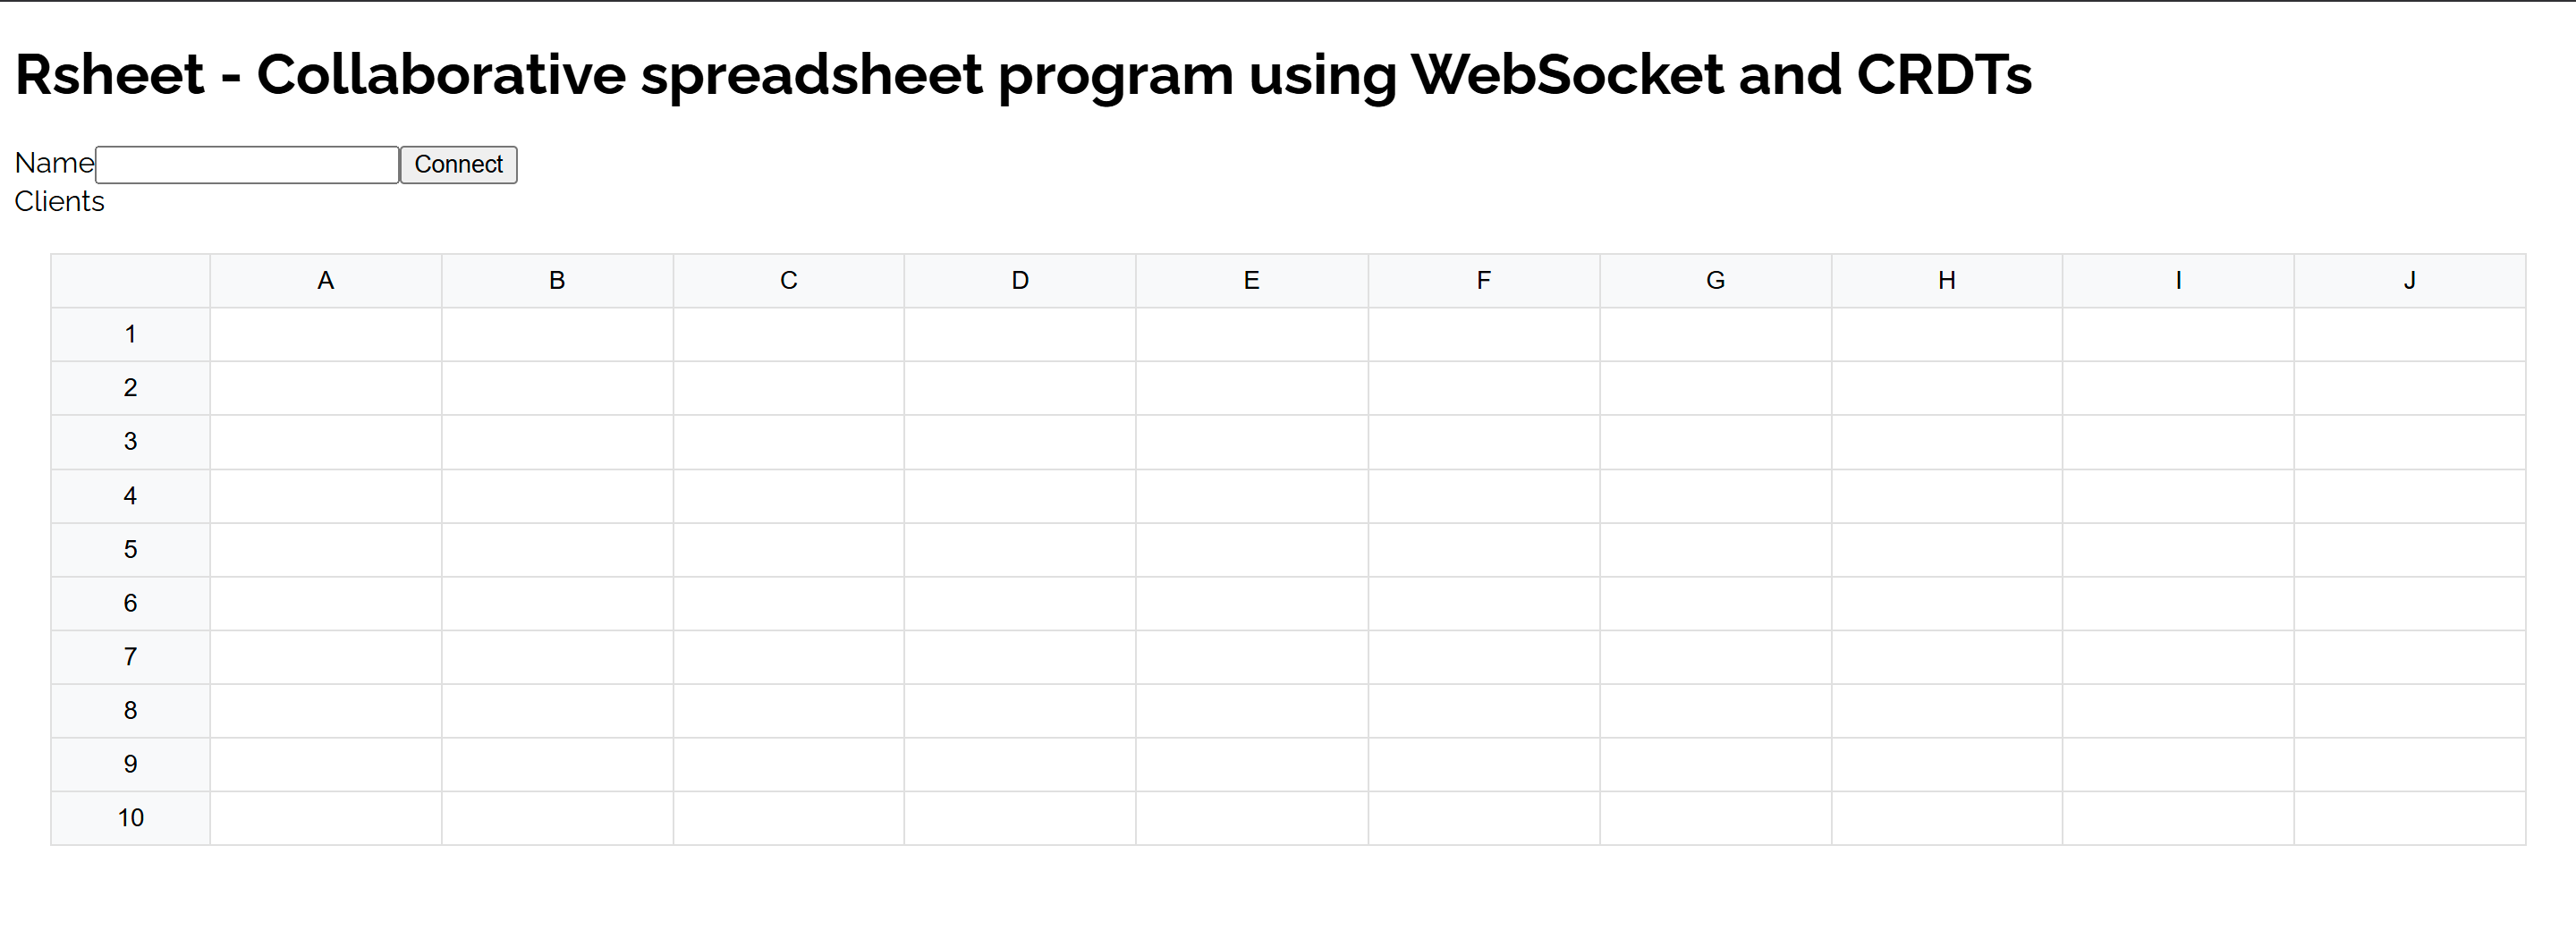
\includegraphics[width=0.75\columnwidth]{figures/crdt1.png}
    		\caption{Frontend of the CRDT-enabled websocket application.}
    		\label{fig:figure}
    	\end{figure}

 	\begin{figure}[H]
    		\centering
    		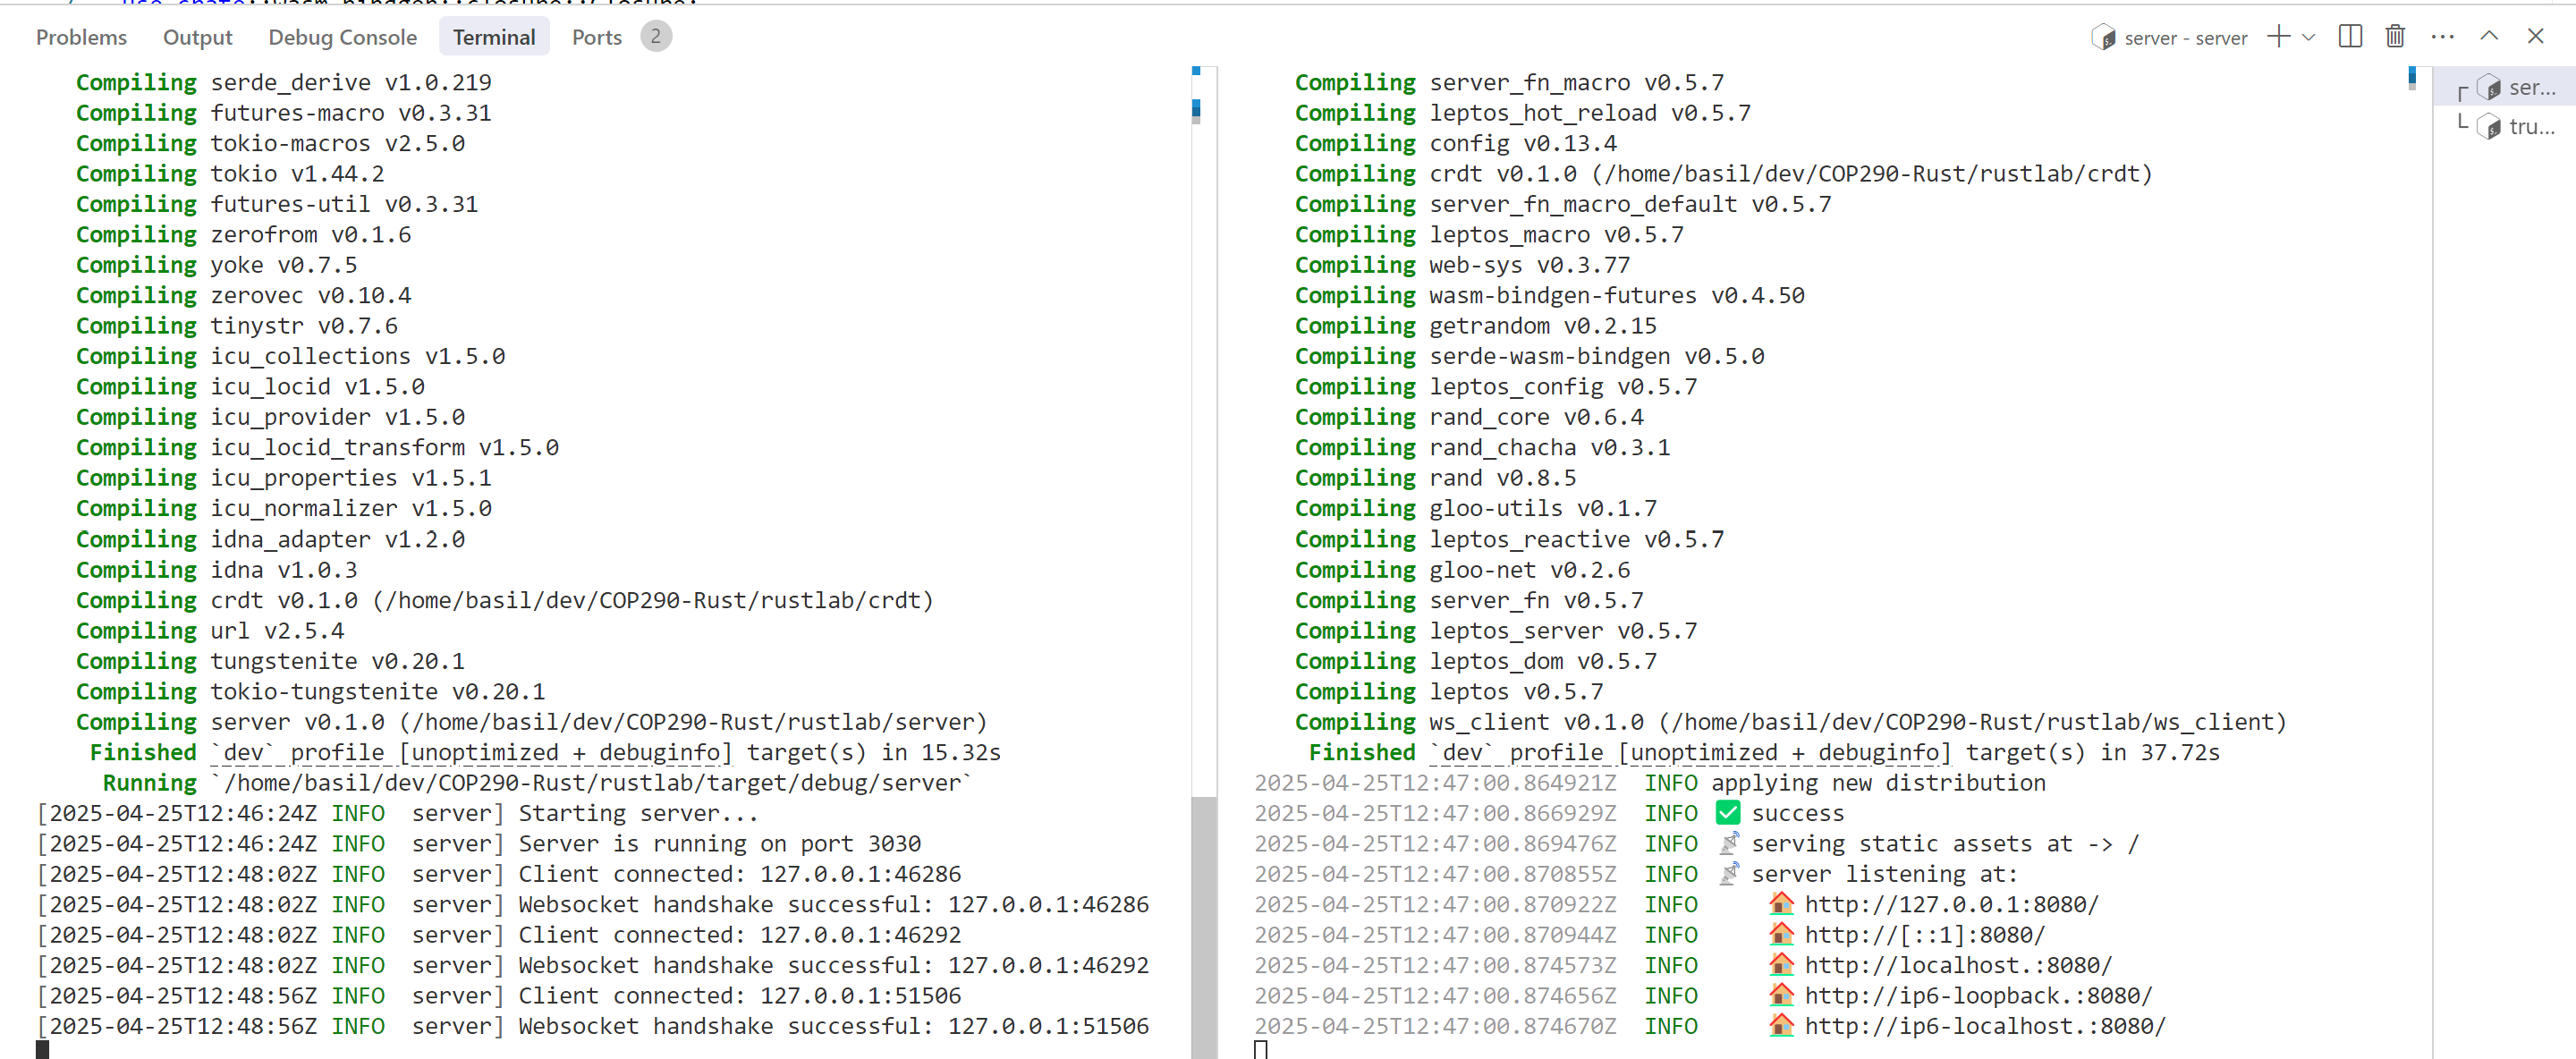
\includegraphics[width=0.75\columnwidth]{figures/crdt2.png}
    		\caption{Screenshot of the terminal showing server and client processes.}
    		\label{fig:figure}
    	\end{figure}

        \begin{figure}[H]
    		\centering
    		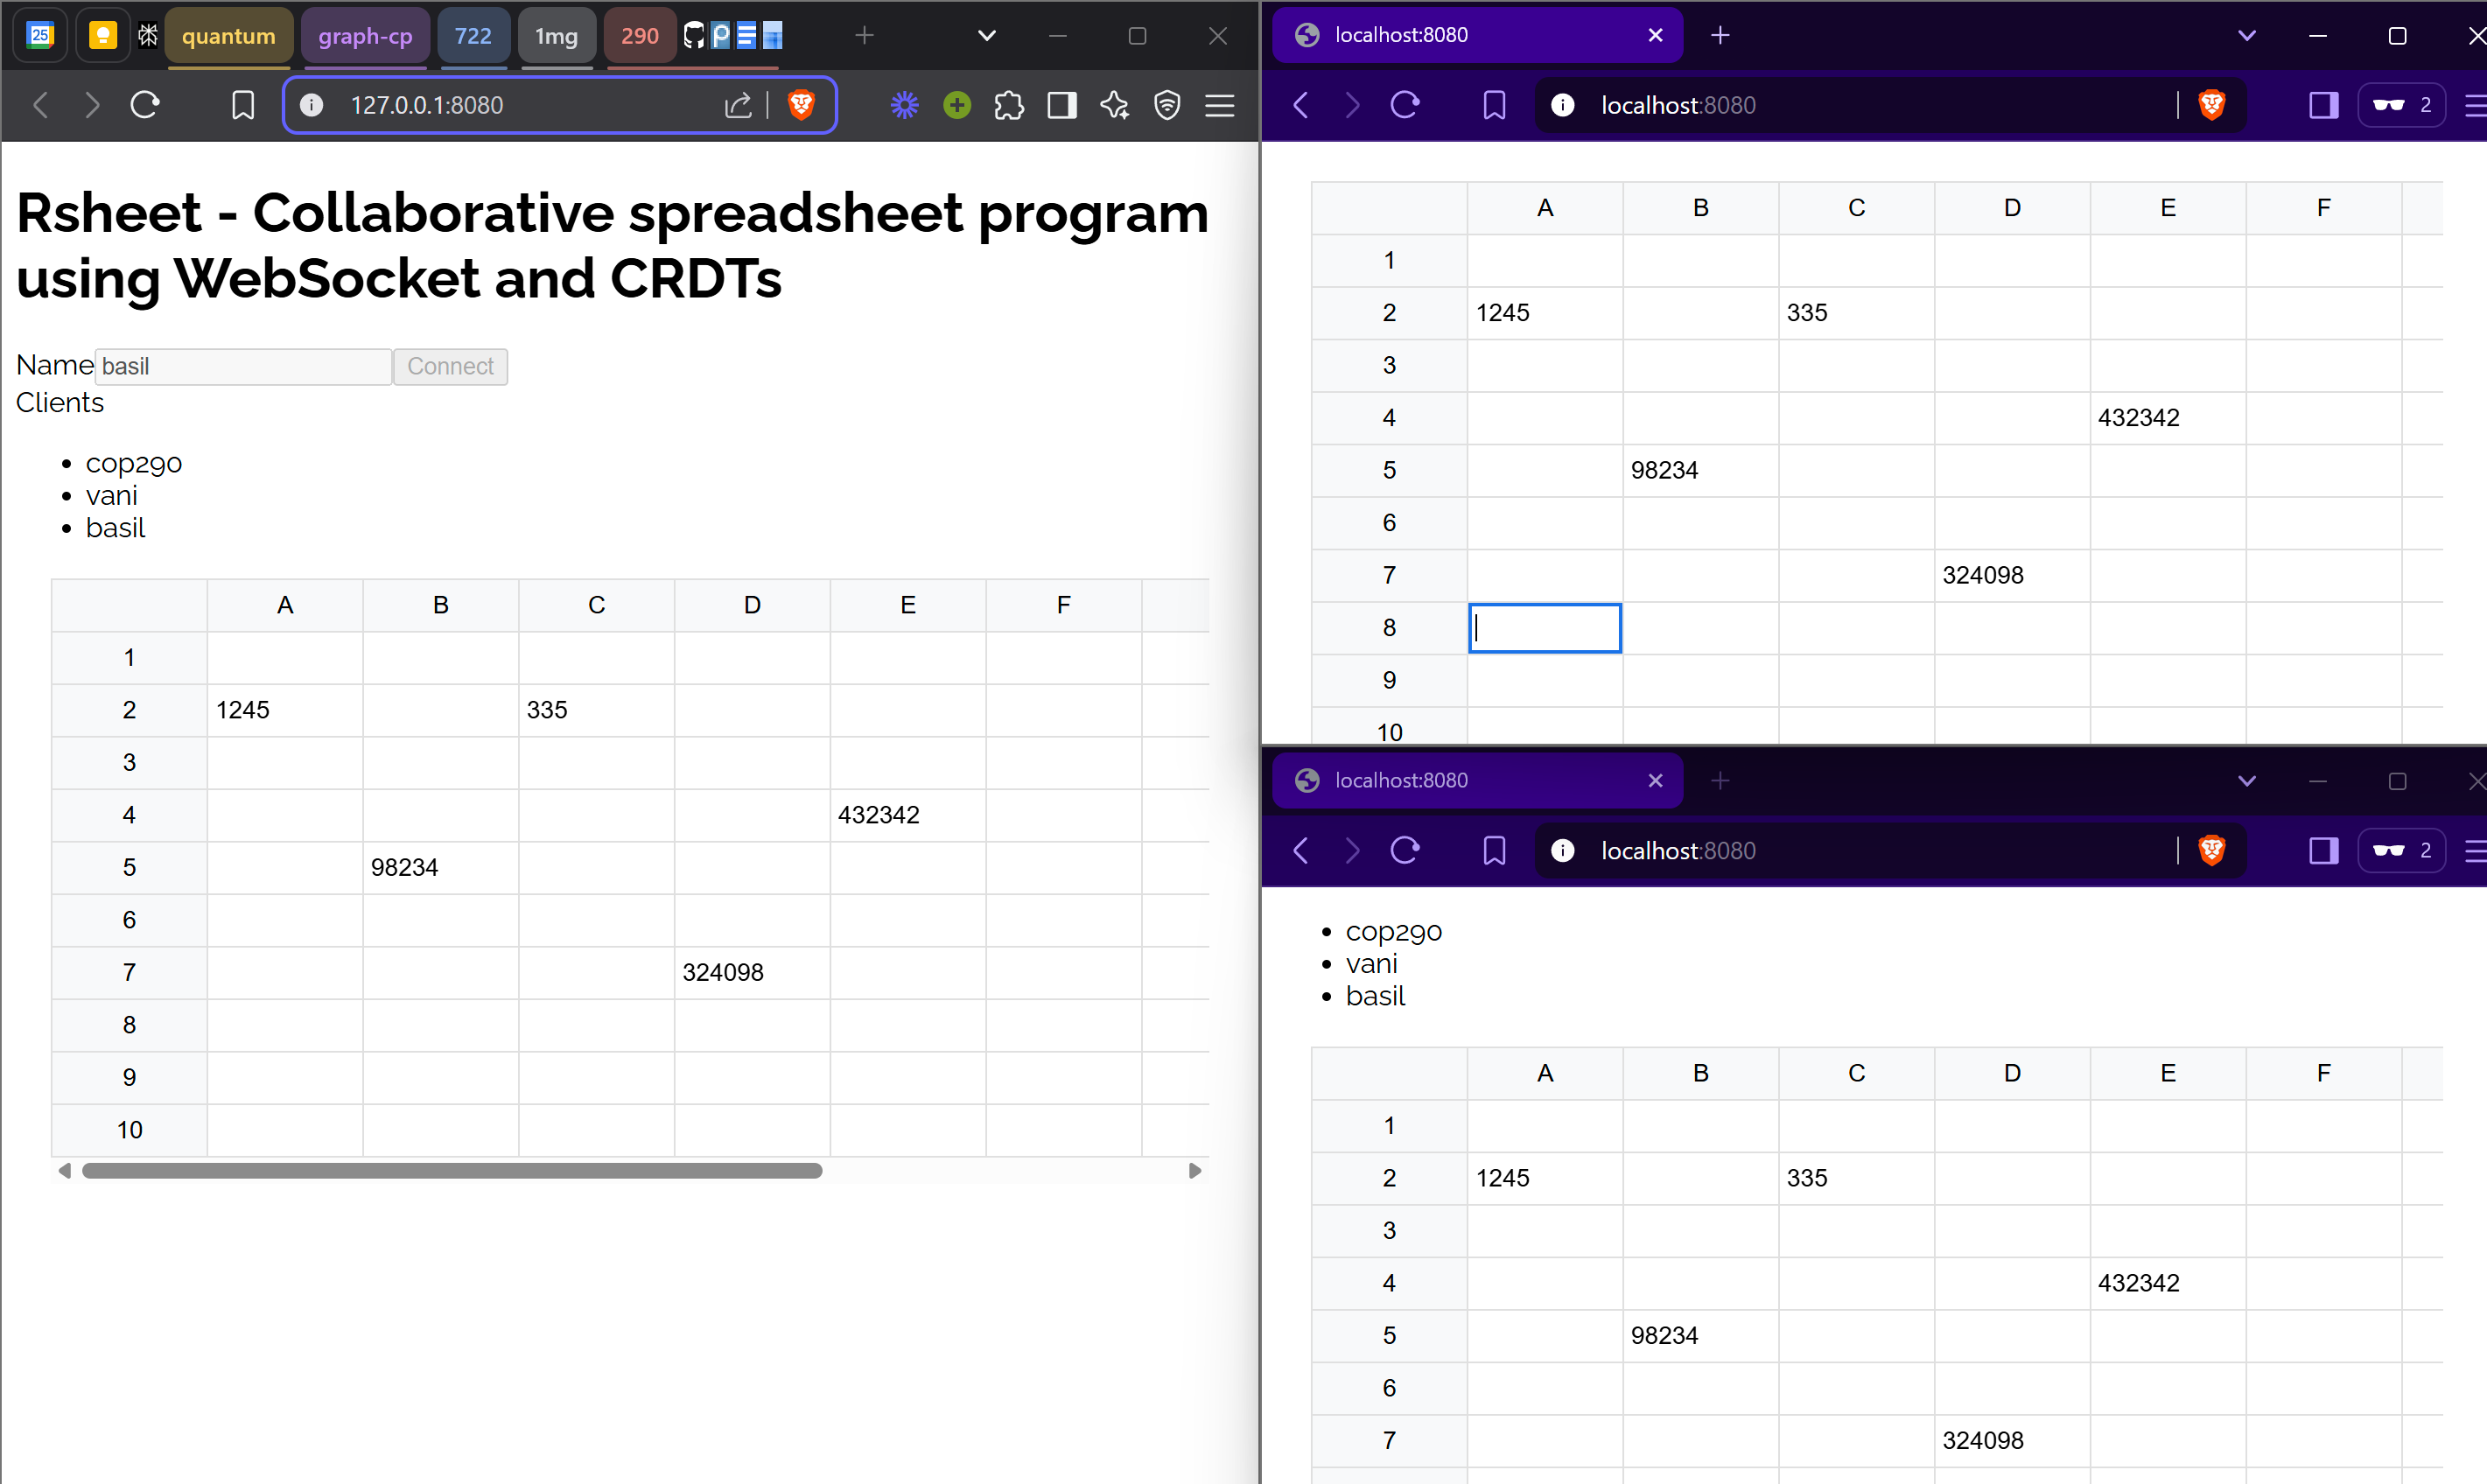
\includegraphics[width=0.75\columnwidth]{figures/crdt3.png}
    		\caption{Screenshot showing multiple users interacting with the same spreadsheet.}
    		\label{fig:figure}
    	\end{figure}

\subsection{Client-Server based GUI Application}

 	\begin{figure}[H]
    		\centering
    		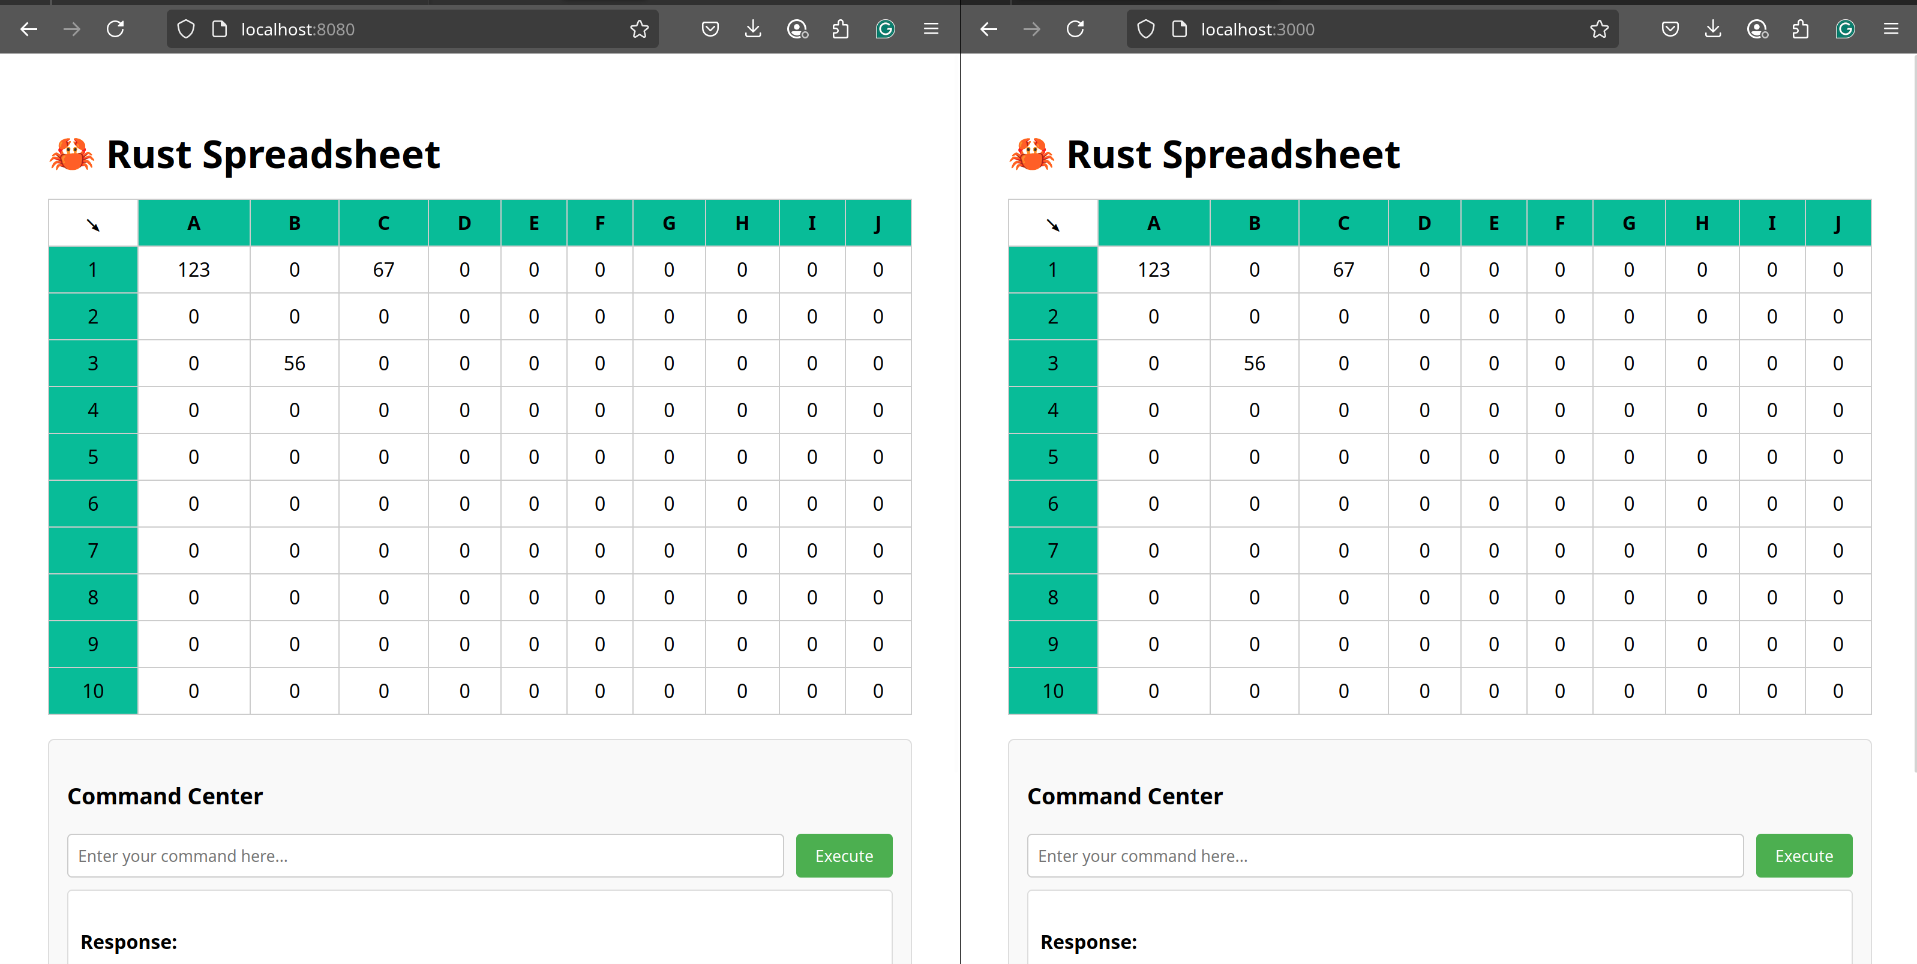
\includegraphics[width=0.75\columnwidth]{figures/2_servers_gui.png}
    		\caption{Screenshot of multiple clients.}
    		\label{fig:figure}
    	\end{figure}

        \begin{figure}[H]
            \centering
            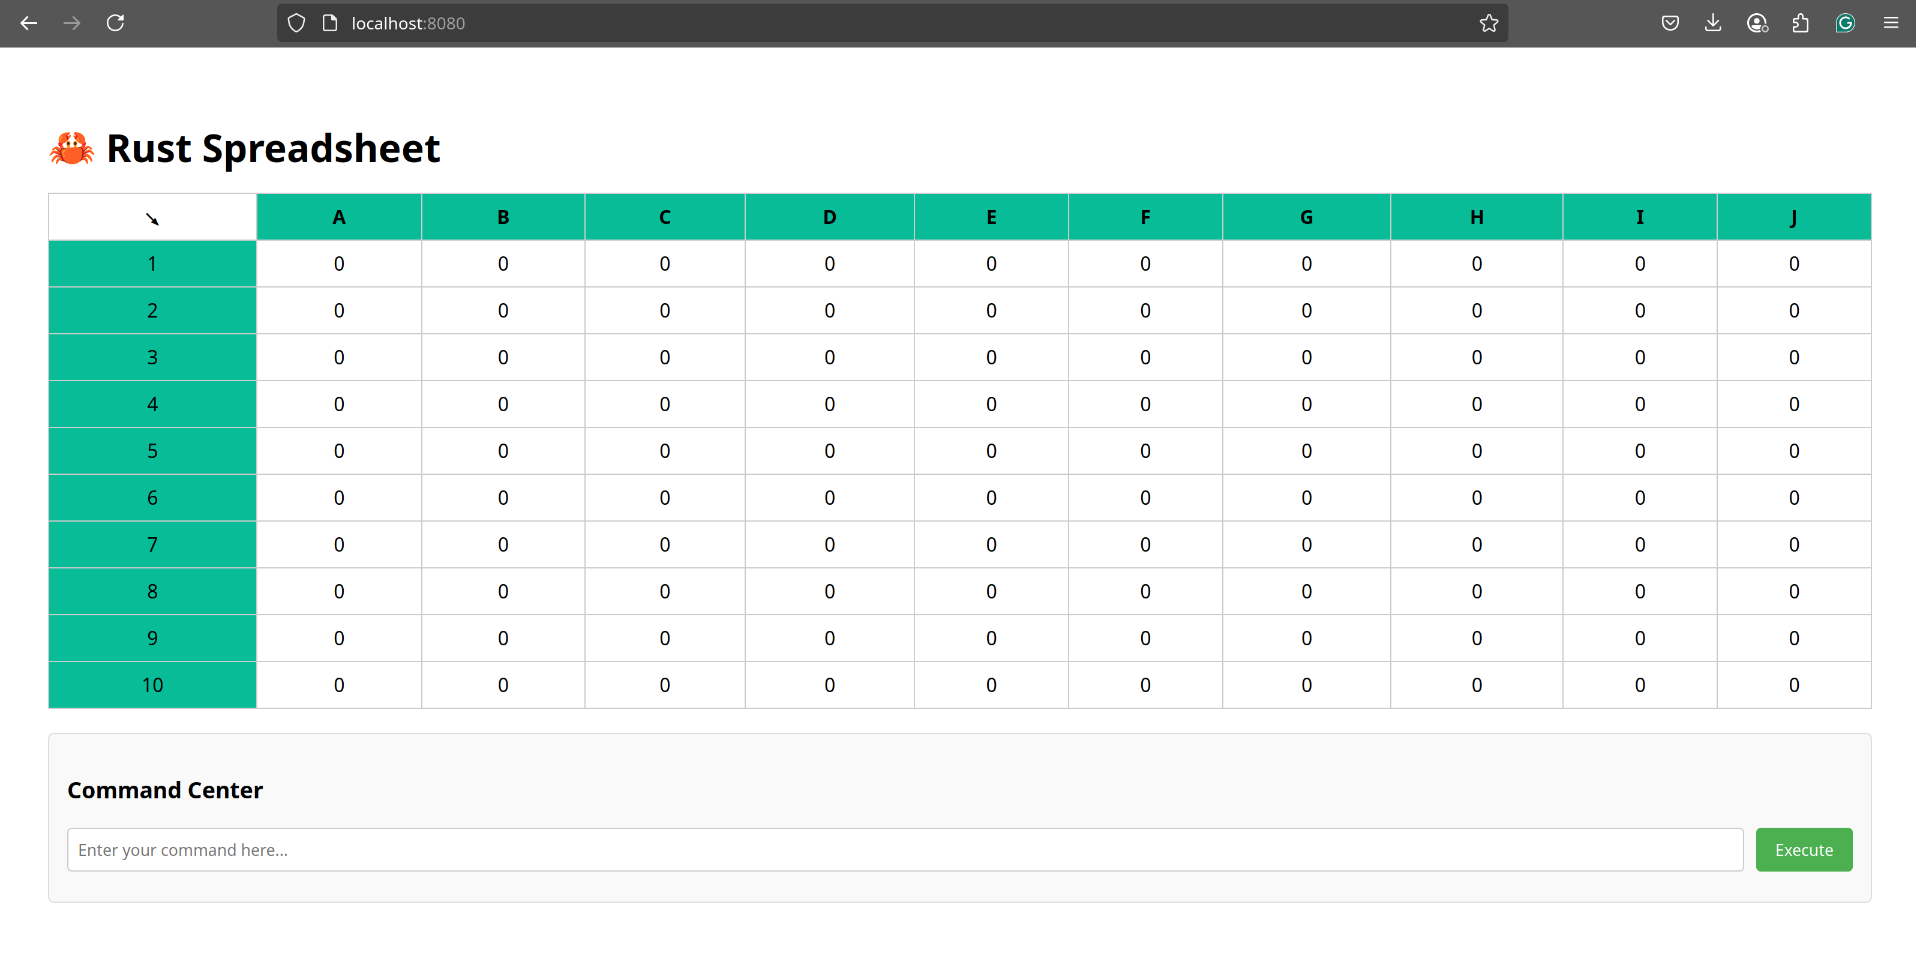
\includegraphics[width=0.75\linewidth]{figures/Web_GUI.png}
            \caption{Showcasing Web GUI}
            \label{fig:enter-label}
        \end{figure}

        \begin{figure}[H]
            \centering
            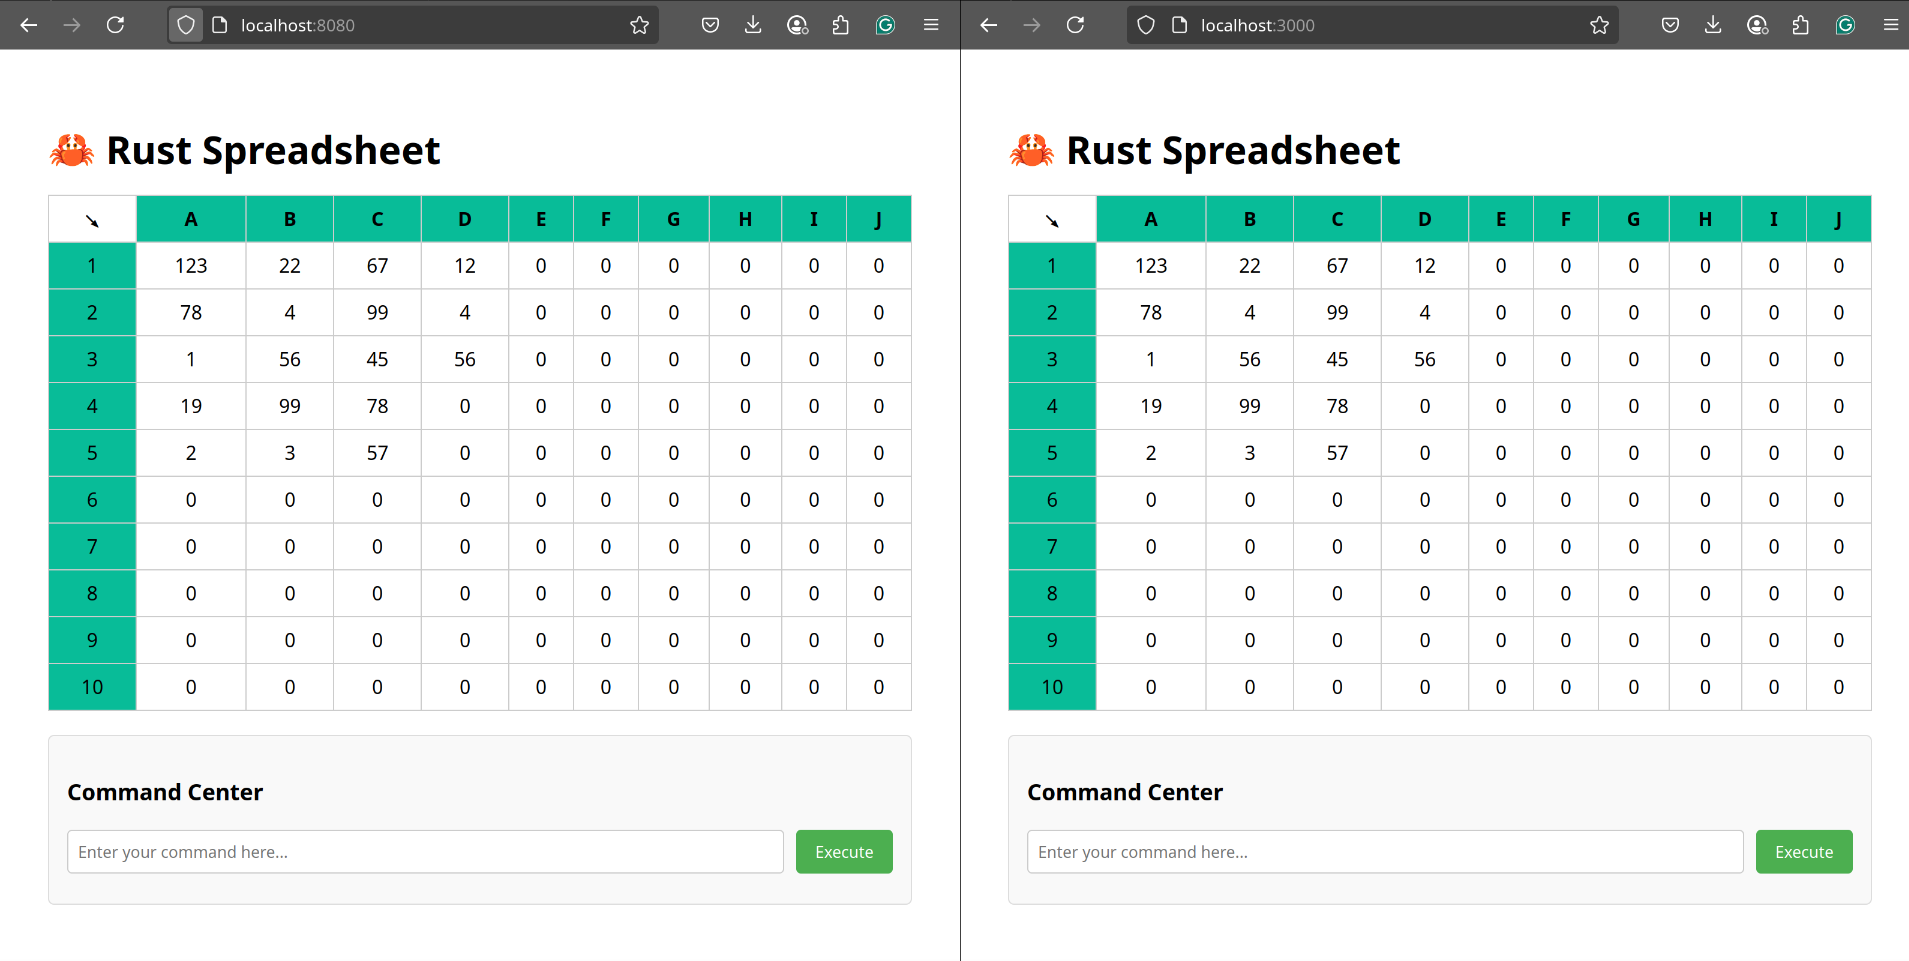
\includegraphics[width=0.75\linewidth]{figures/sync_data_gui.png}
            \caption{Synchronizing data between different clients}
            \label{fig:enter-label}
        \end{figure}

\subsection{Extended TUI Application}

        \begin{figure}[H]
            \centering
            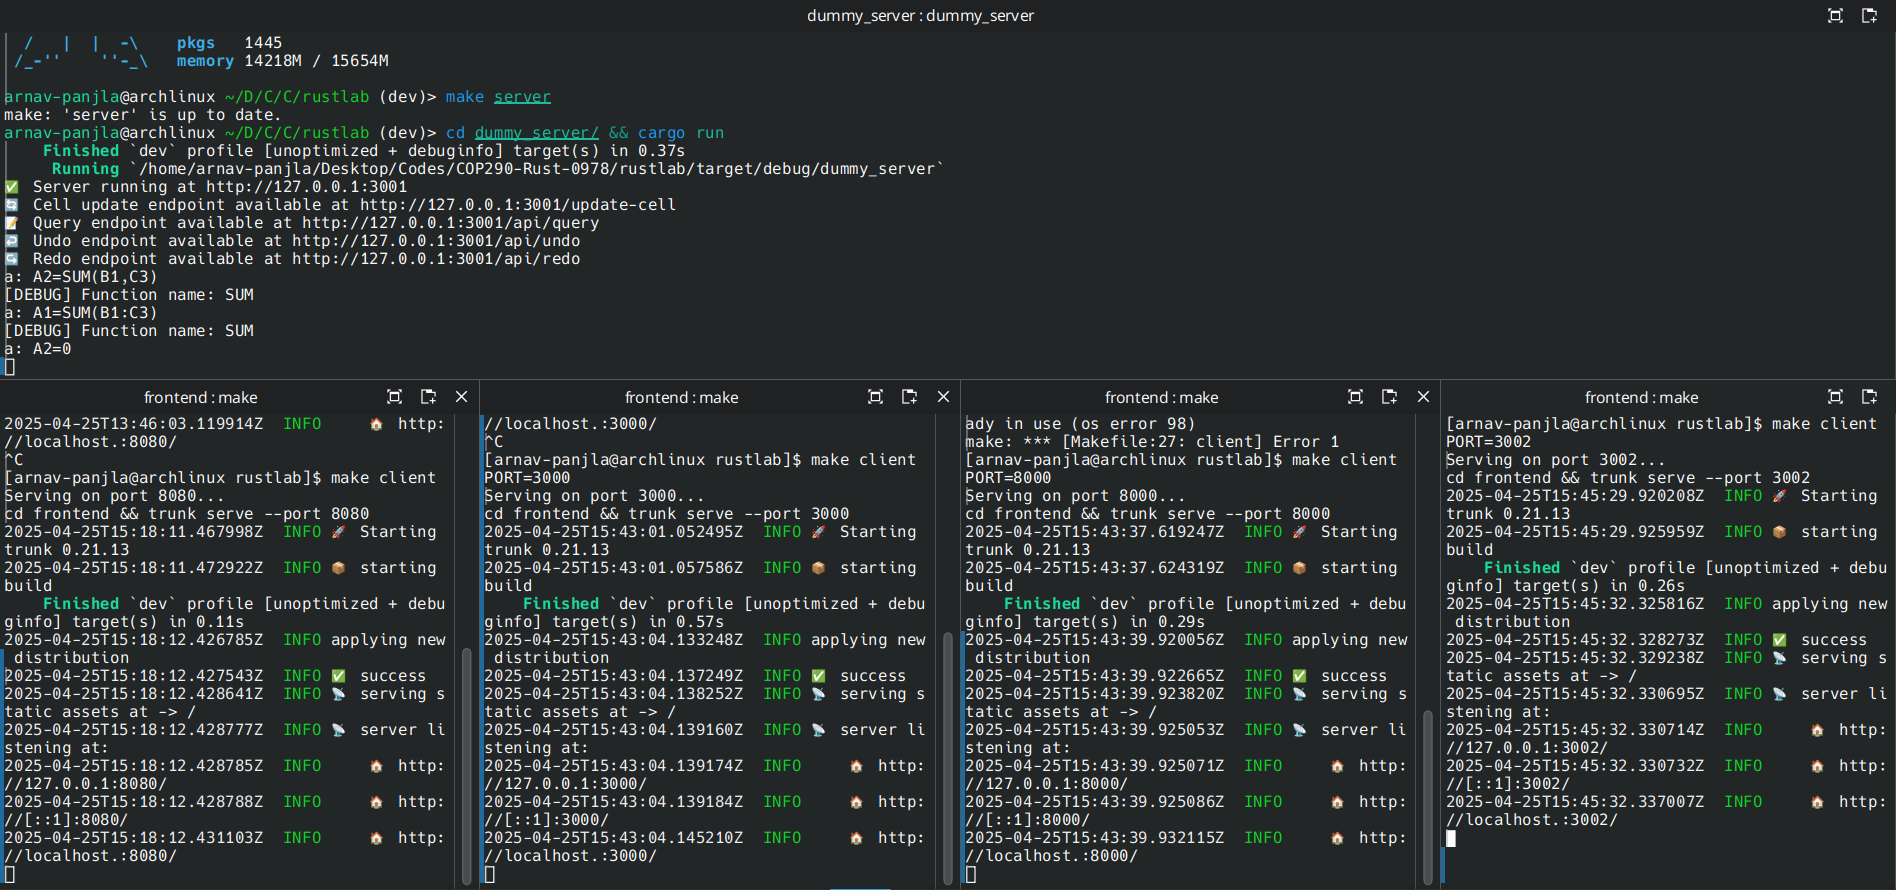
\includegraphics[width=0.75\linewidth]{figures/runnning_multiple_clients.png}
            \caption{Running multiple clients}
            \label{fig:enter-label}
        \end{figure}

        \begin{figure}[H]
            \centering
            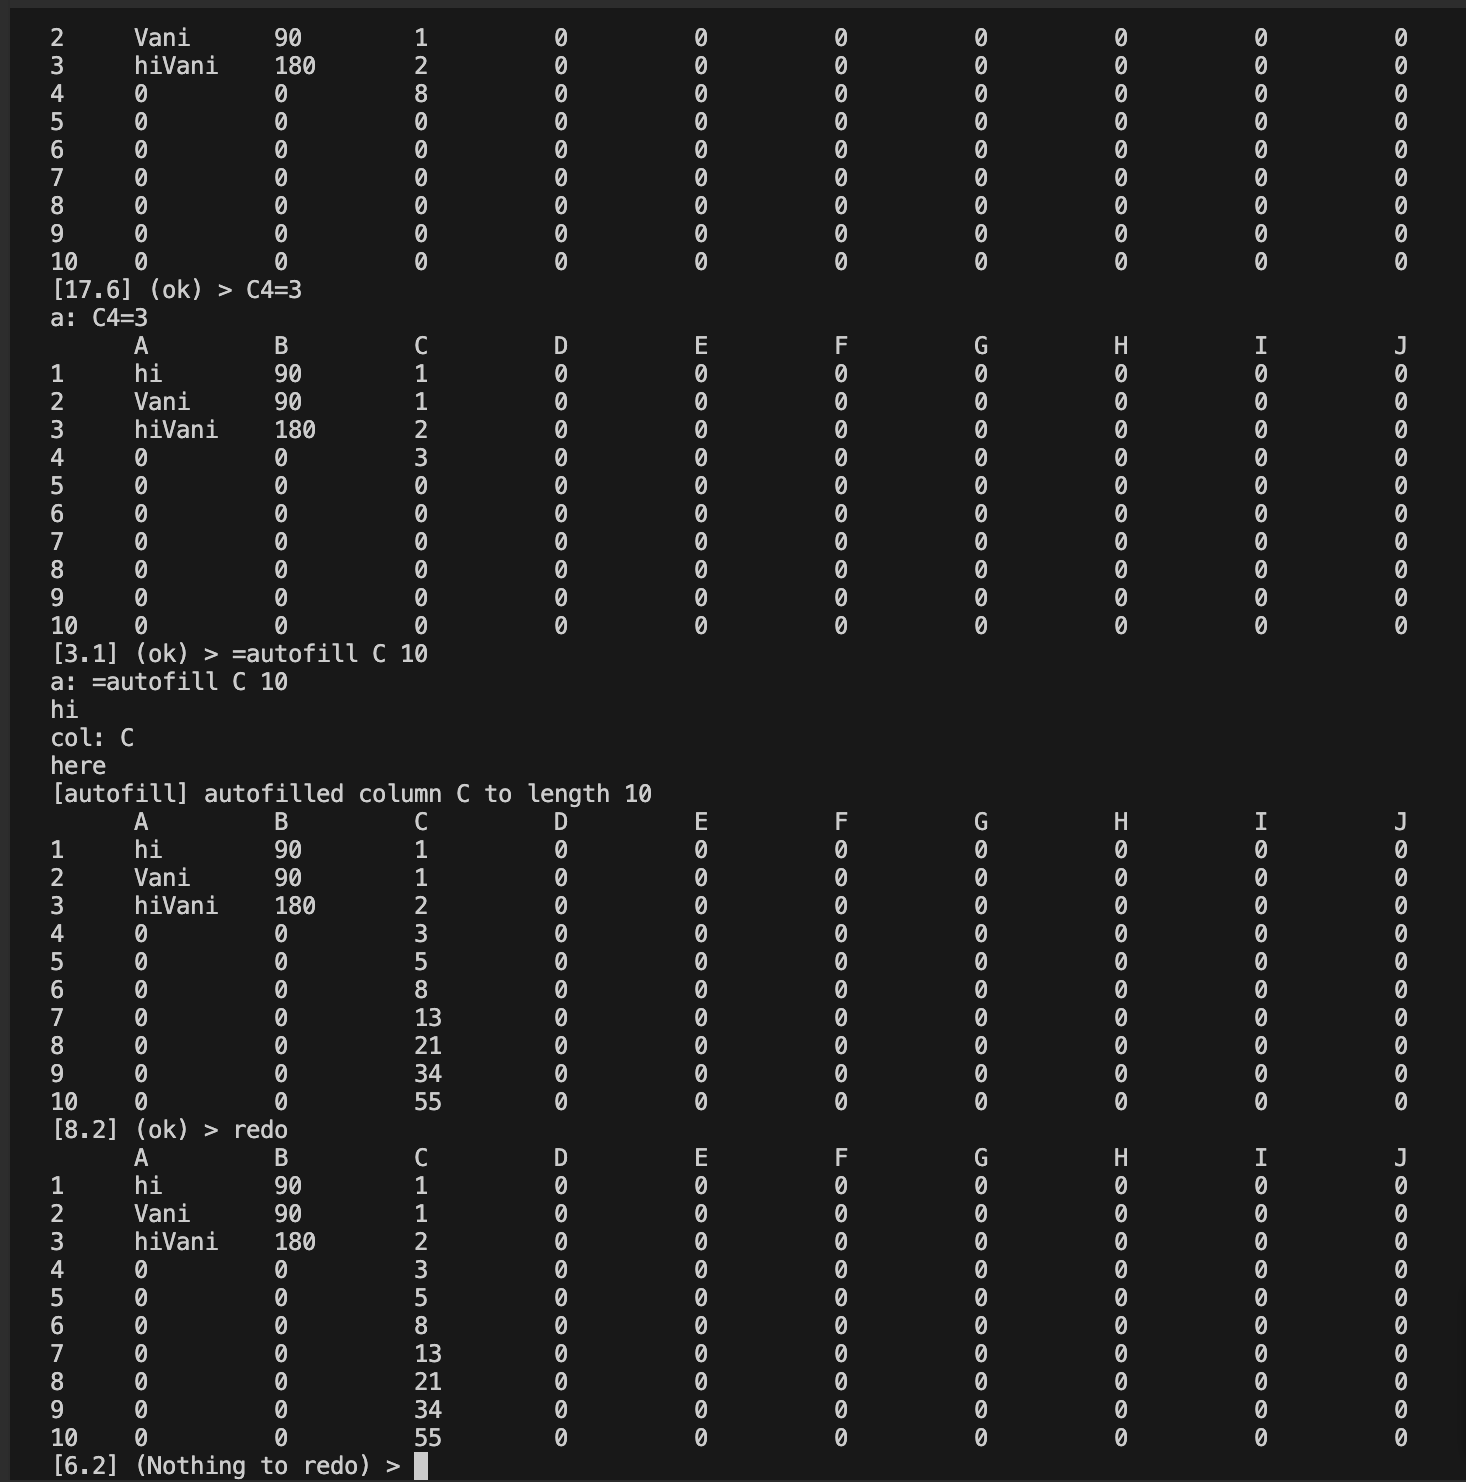
\includegraphics[width=0.5\linewidth]{image.png}
            \caption{Performing string concatenation}
            \label{fig:enter-label}
        \end{figure}

        \begin{figure}[H]
            \centering
            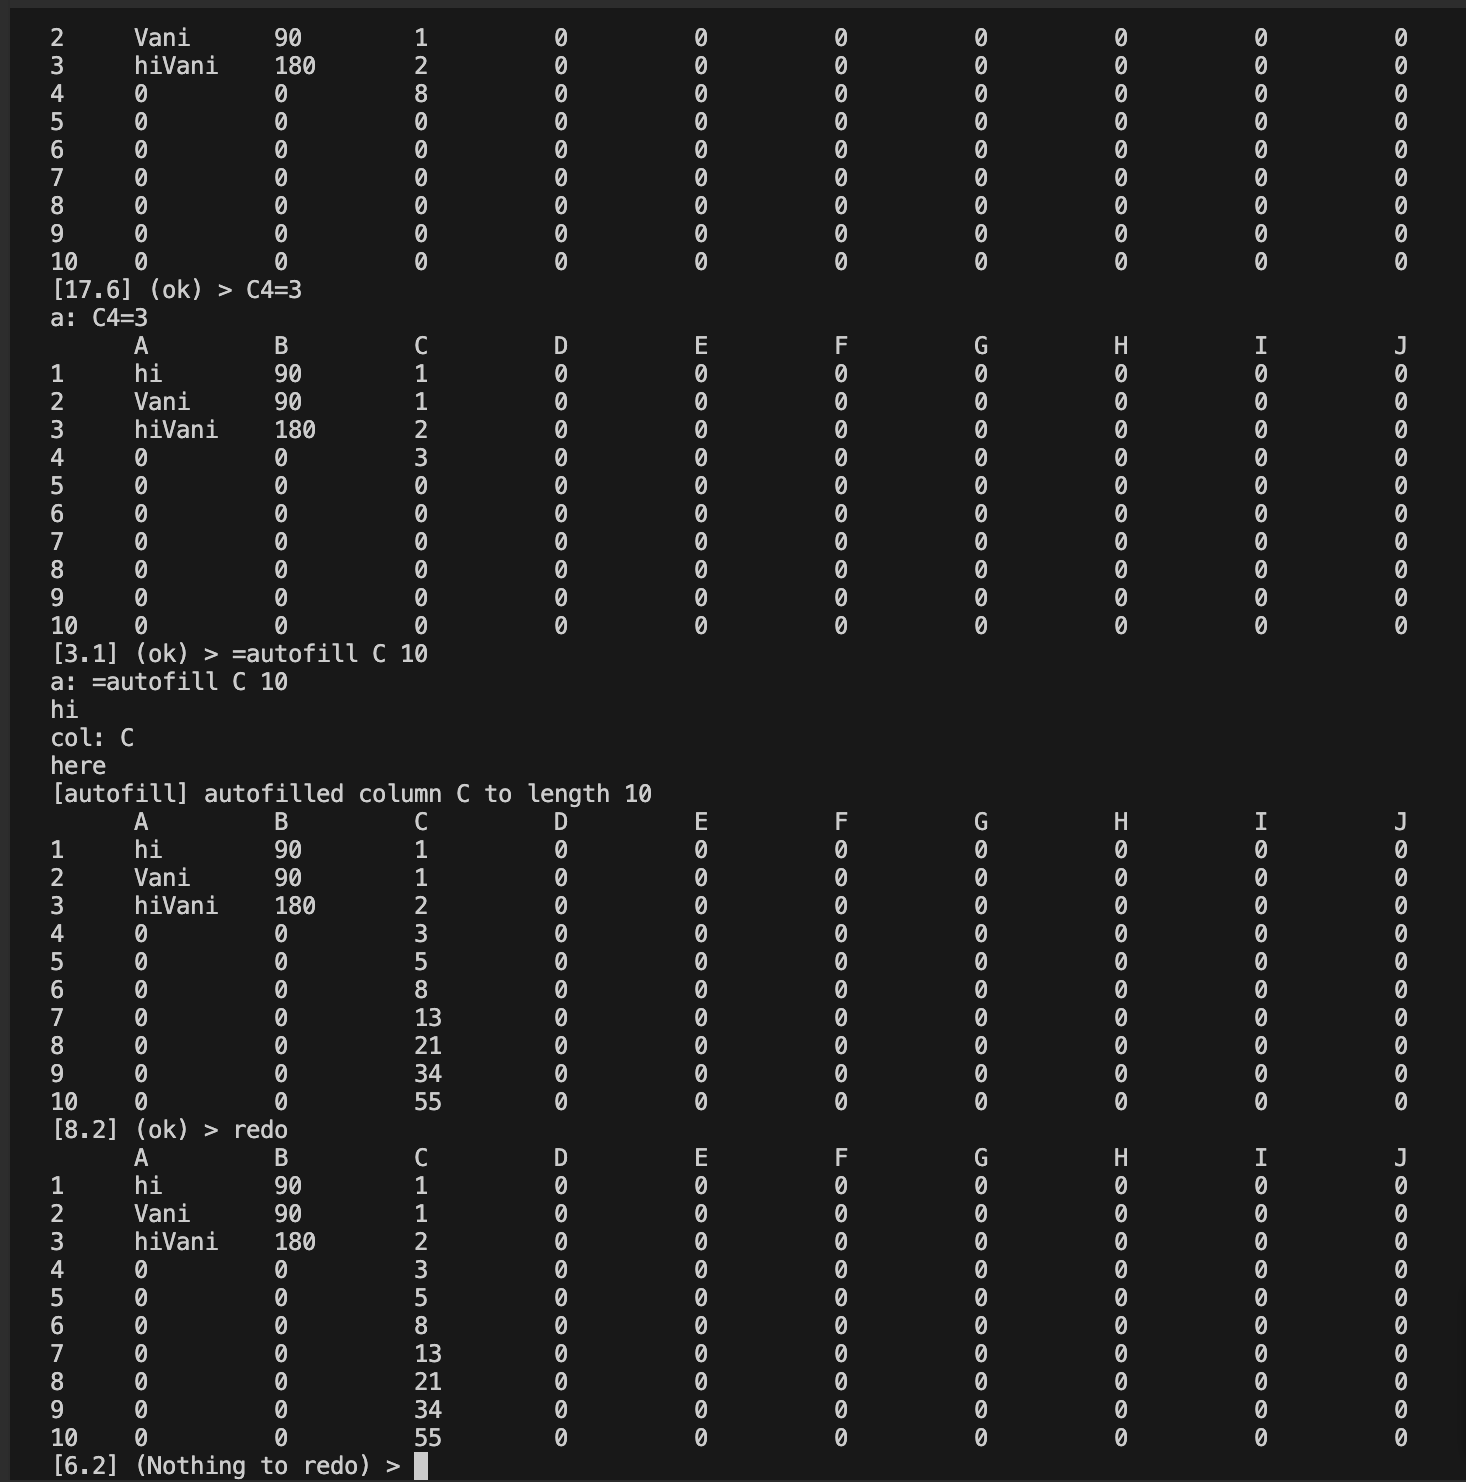
\includegraphics[width=0.5\linewidth]{image.png}
            \caption{Performing recalculation and float-int addition}
            \label{fig:enter-label}
        \end{figure}
        
        \begin{figure}[H]
            \centering
            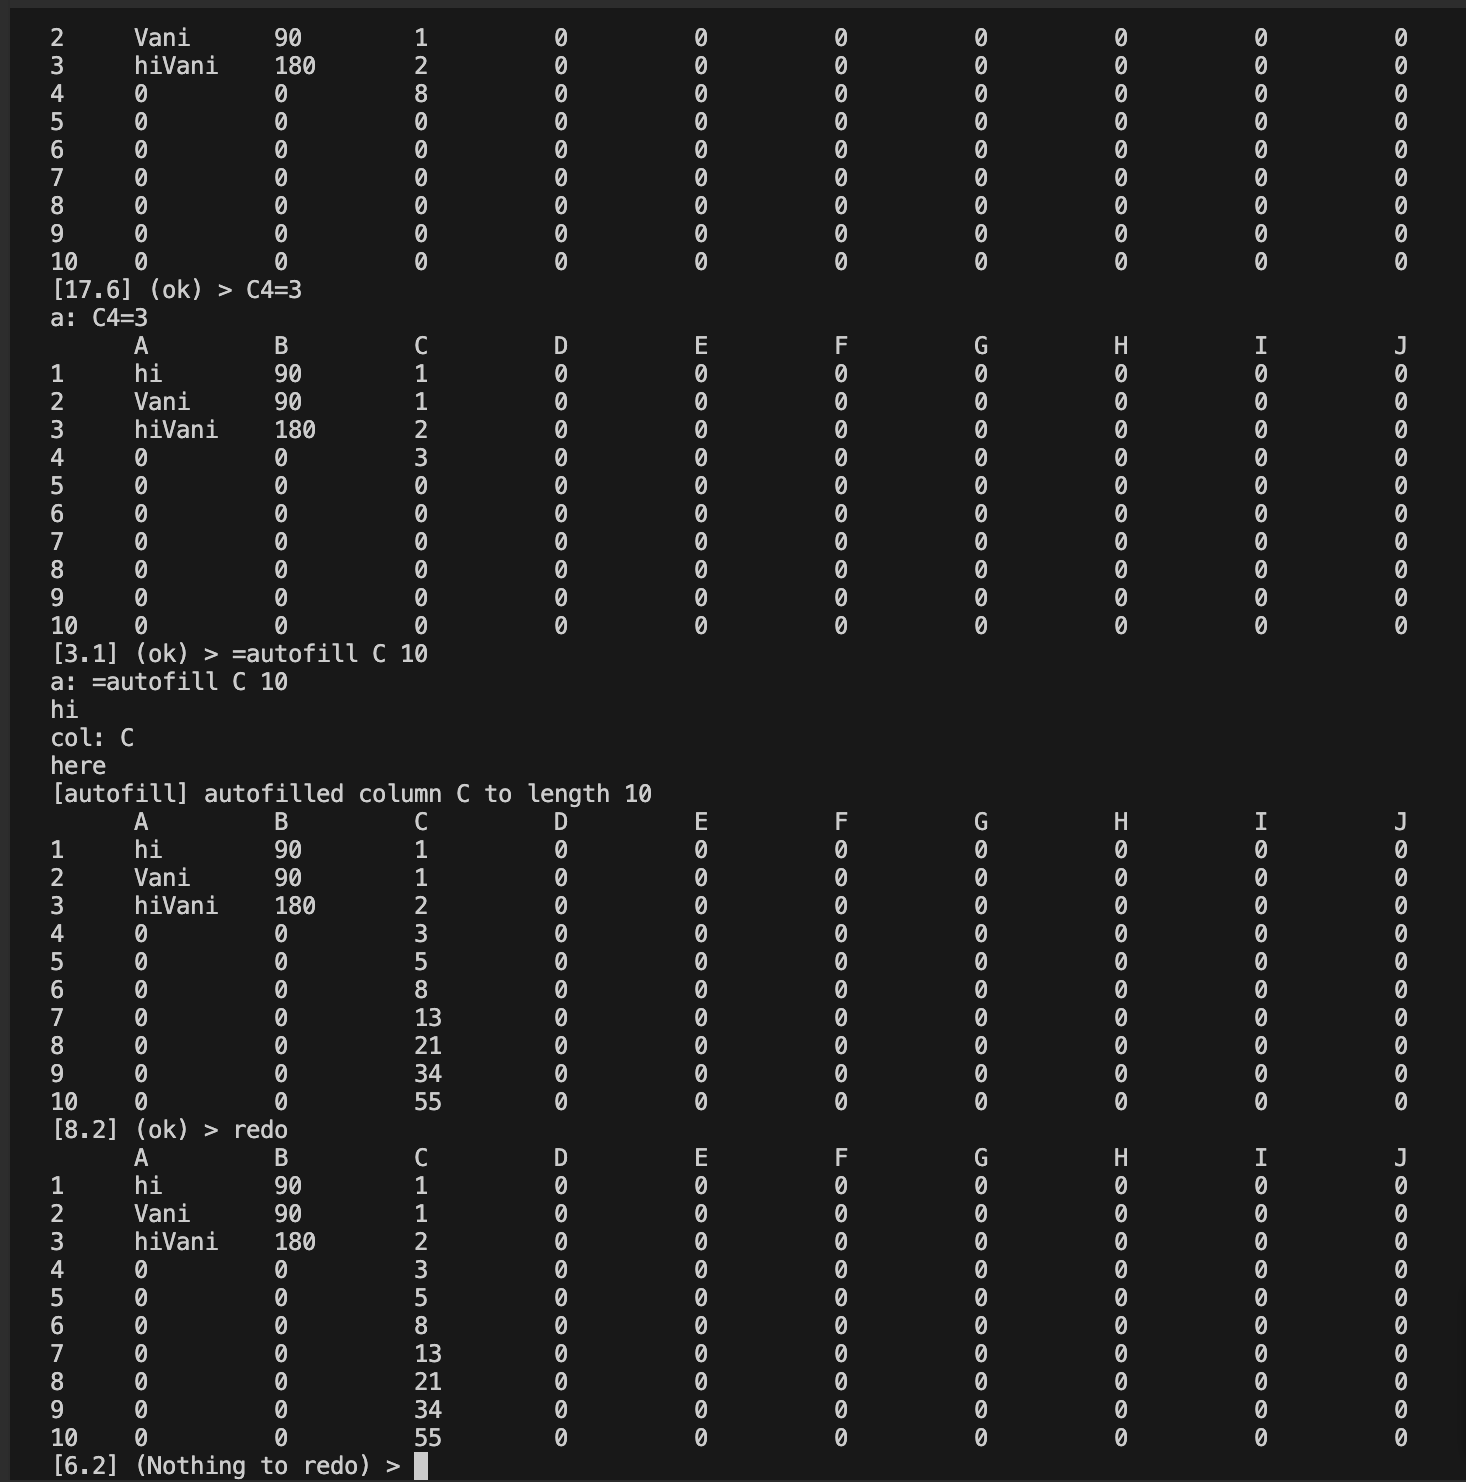
\includegraphics[width=0.5\linewidth]{image.png}
            \caption{Performing recalculation}
            \label{fig:enter-label}
        \end{figure}
        
        \begin{figure}[H]
            \centering
            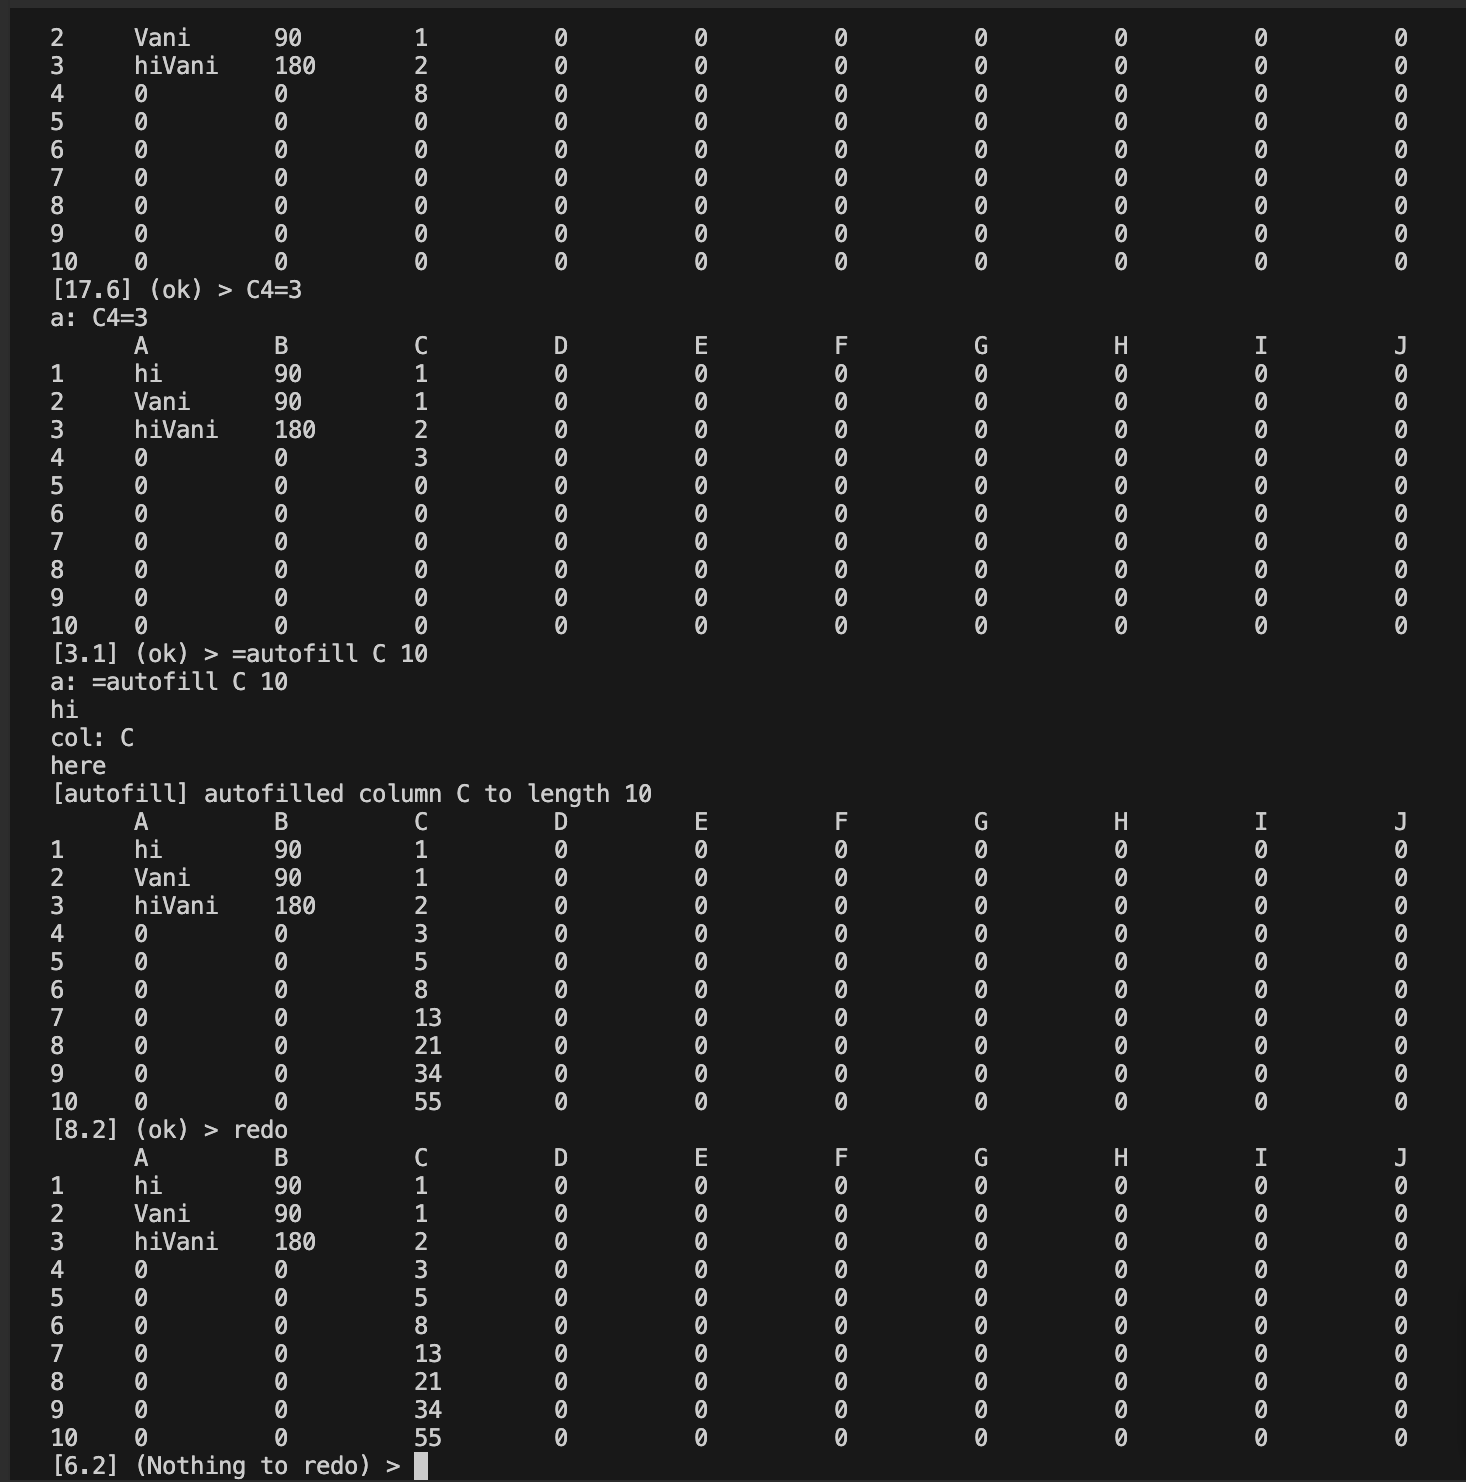
\includegraphics[width=0.5\linewidth]{image.png}
            \caption{Performing autofill for AP series, and undo}
            \label{fig:enter-label}
        \end{figure}
        
        \begin{figure}[H]
            \centering
            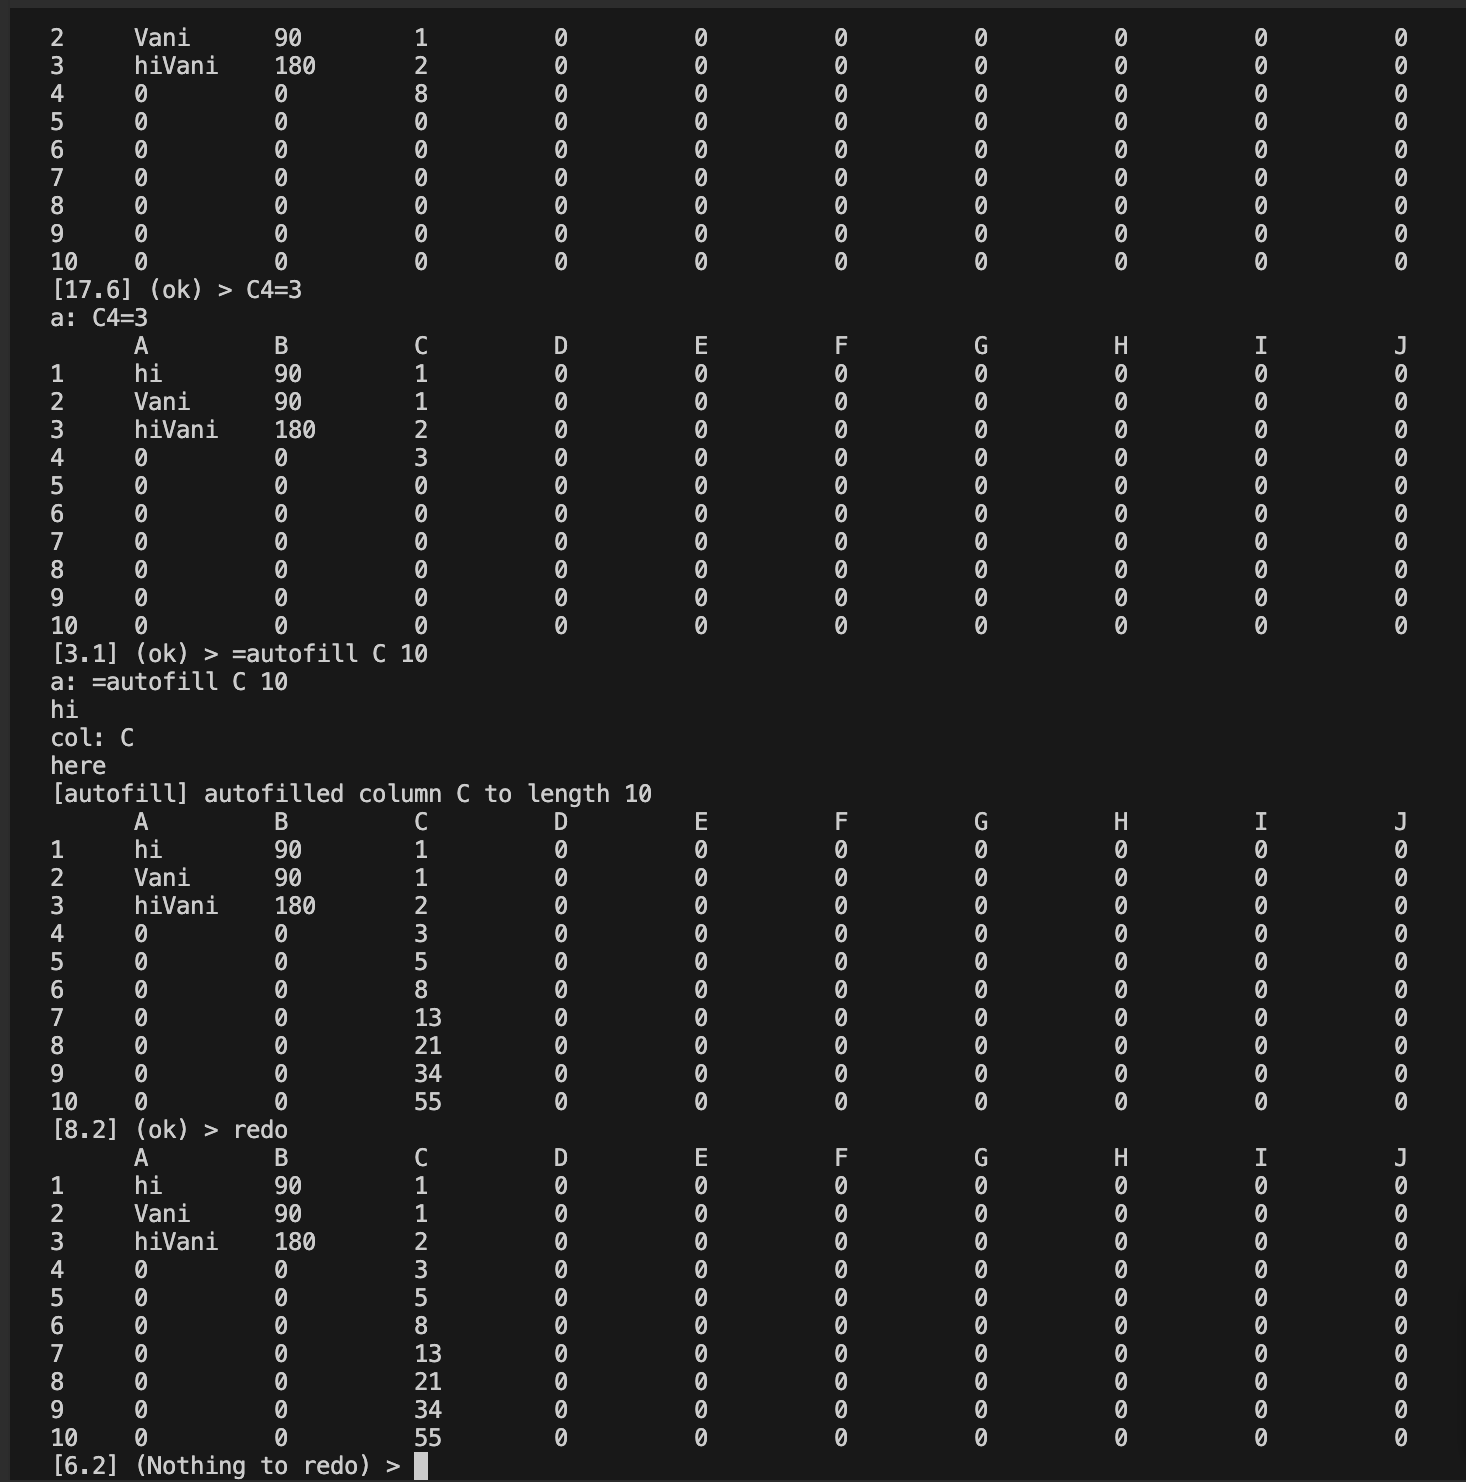
\includegraphics[width=0.5\linewidth]{image.png}
            \caption{Performing undo}
            \label{fig:enter-label}
        \end{figure}
        
        \begin{figure}[H]
            \centering
            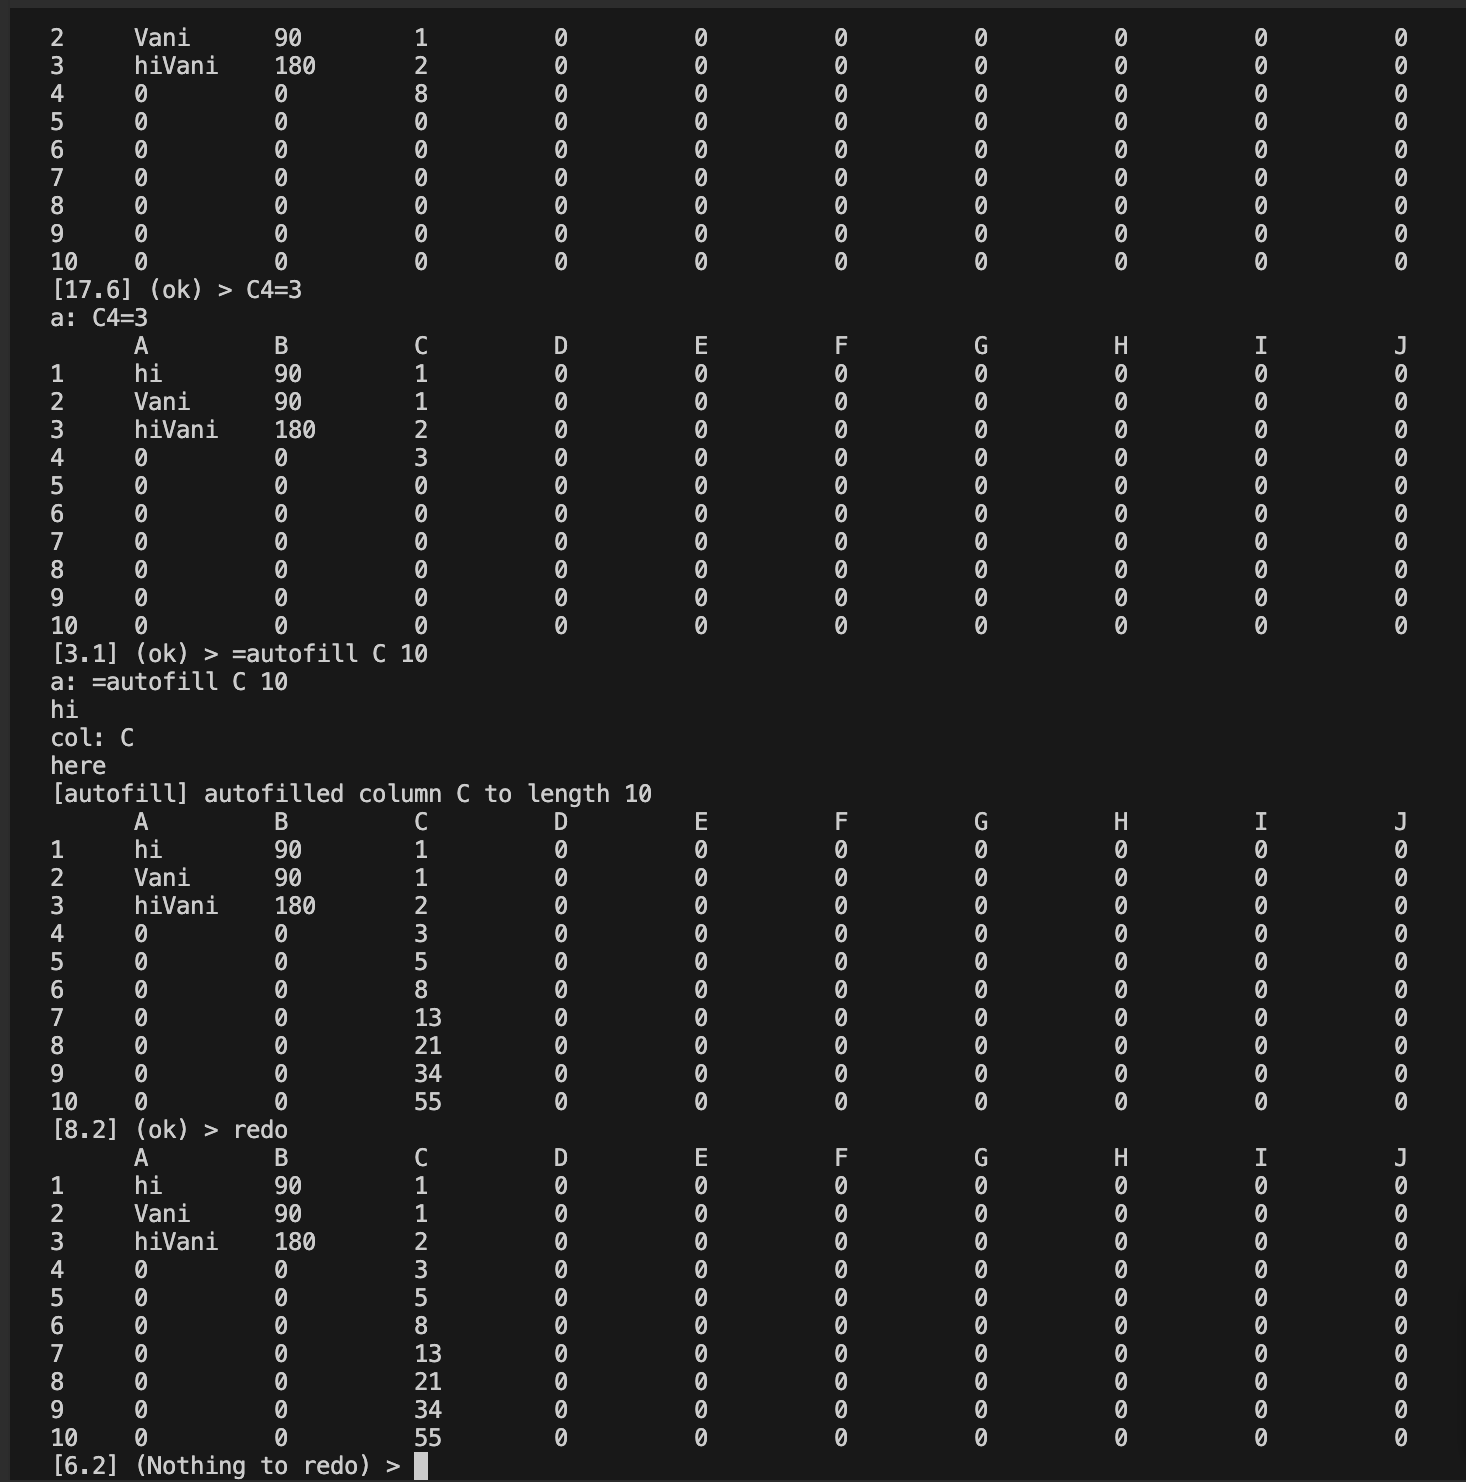
\includegraphics[width=0.5\linewidth]{image.png}
            \caption{Performing redo}
            \label{fig:enter-label}
        \end{figure}
        
        \begin{figure}[H]
            \centering
            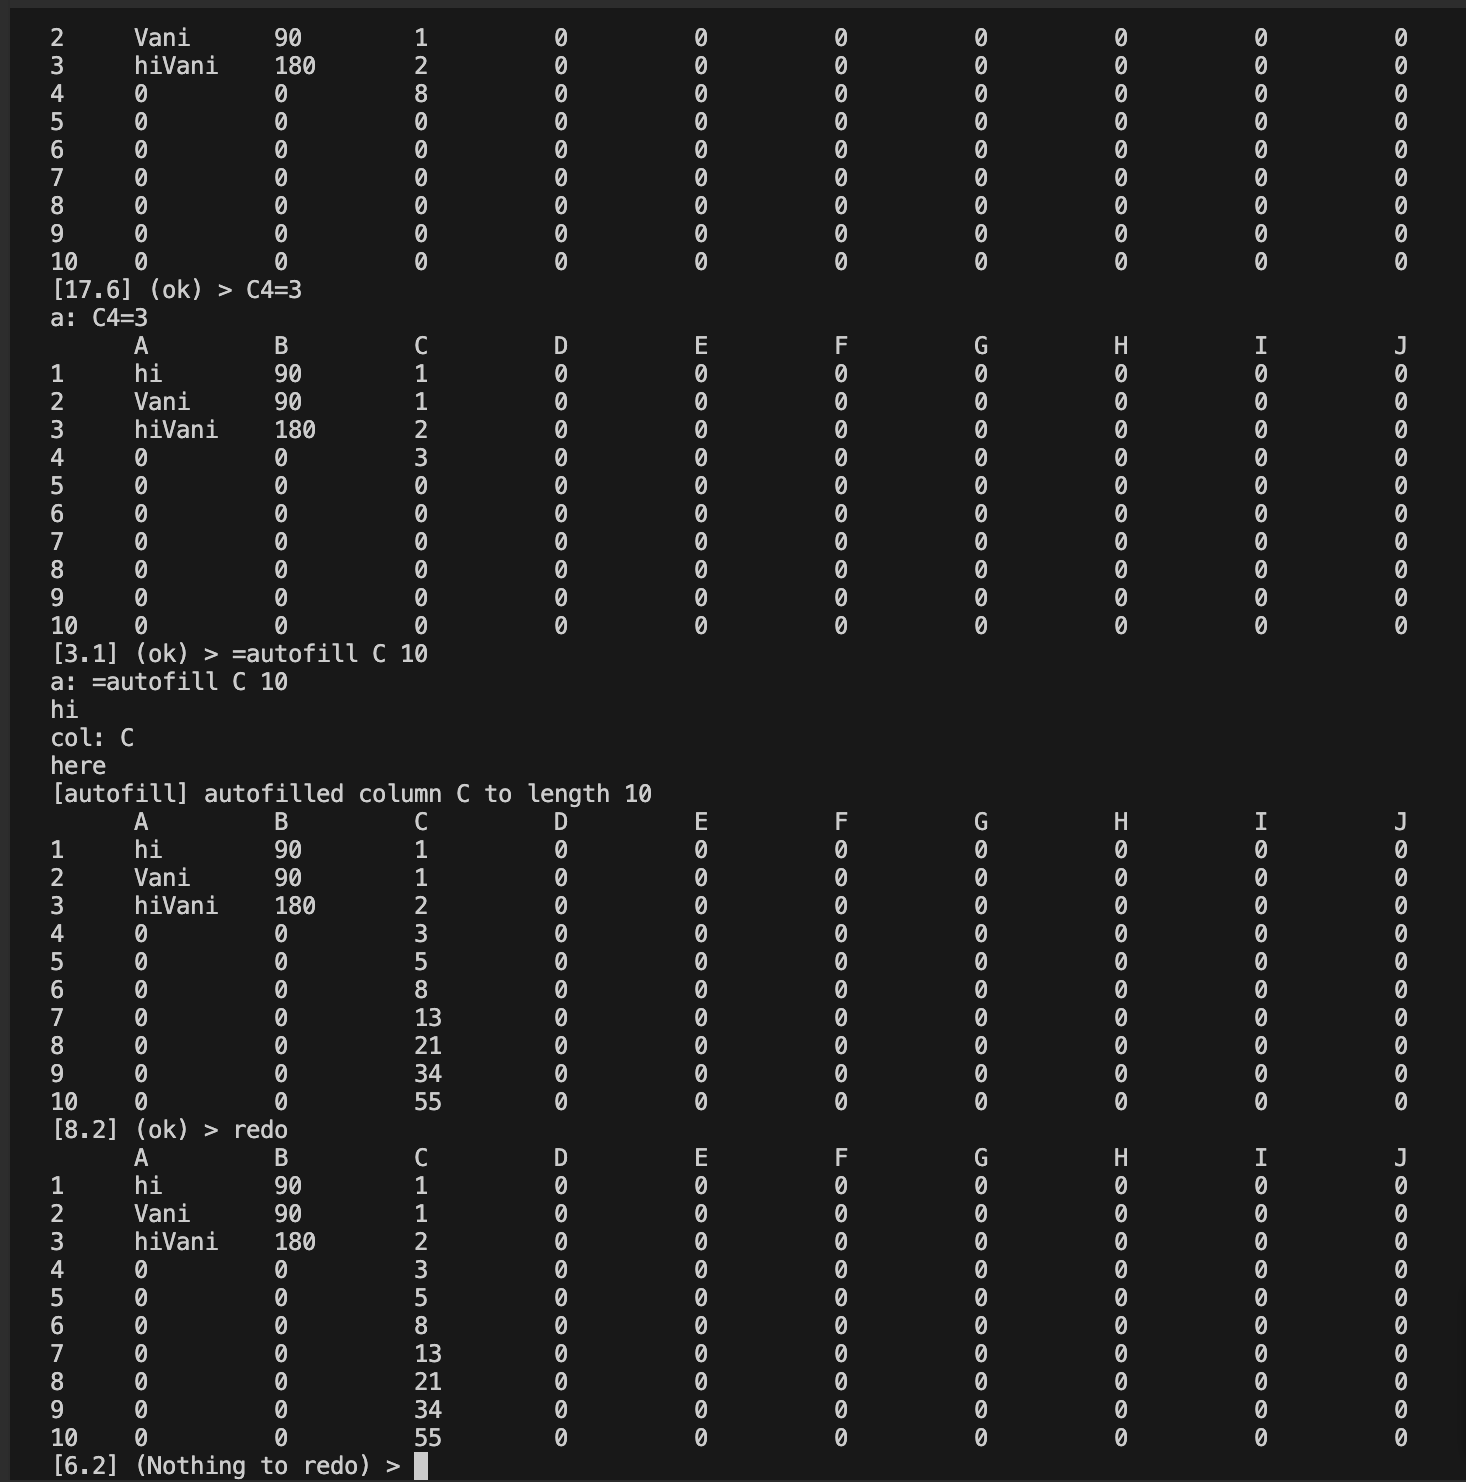
\includegraphics[width=0.5\linewidth]{image.png}
            \caption{Performing autofill for GP}
            \label{fig:enter-label}
        \end{figure}
        
        \begin{figure}[H]
            \centering
            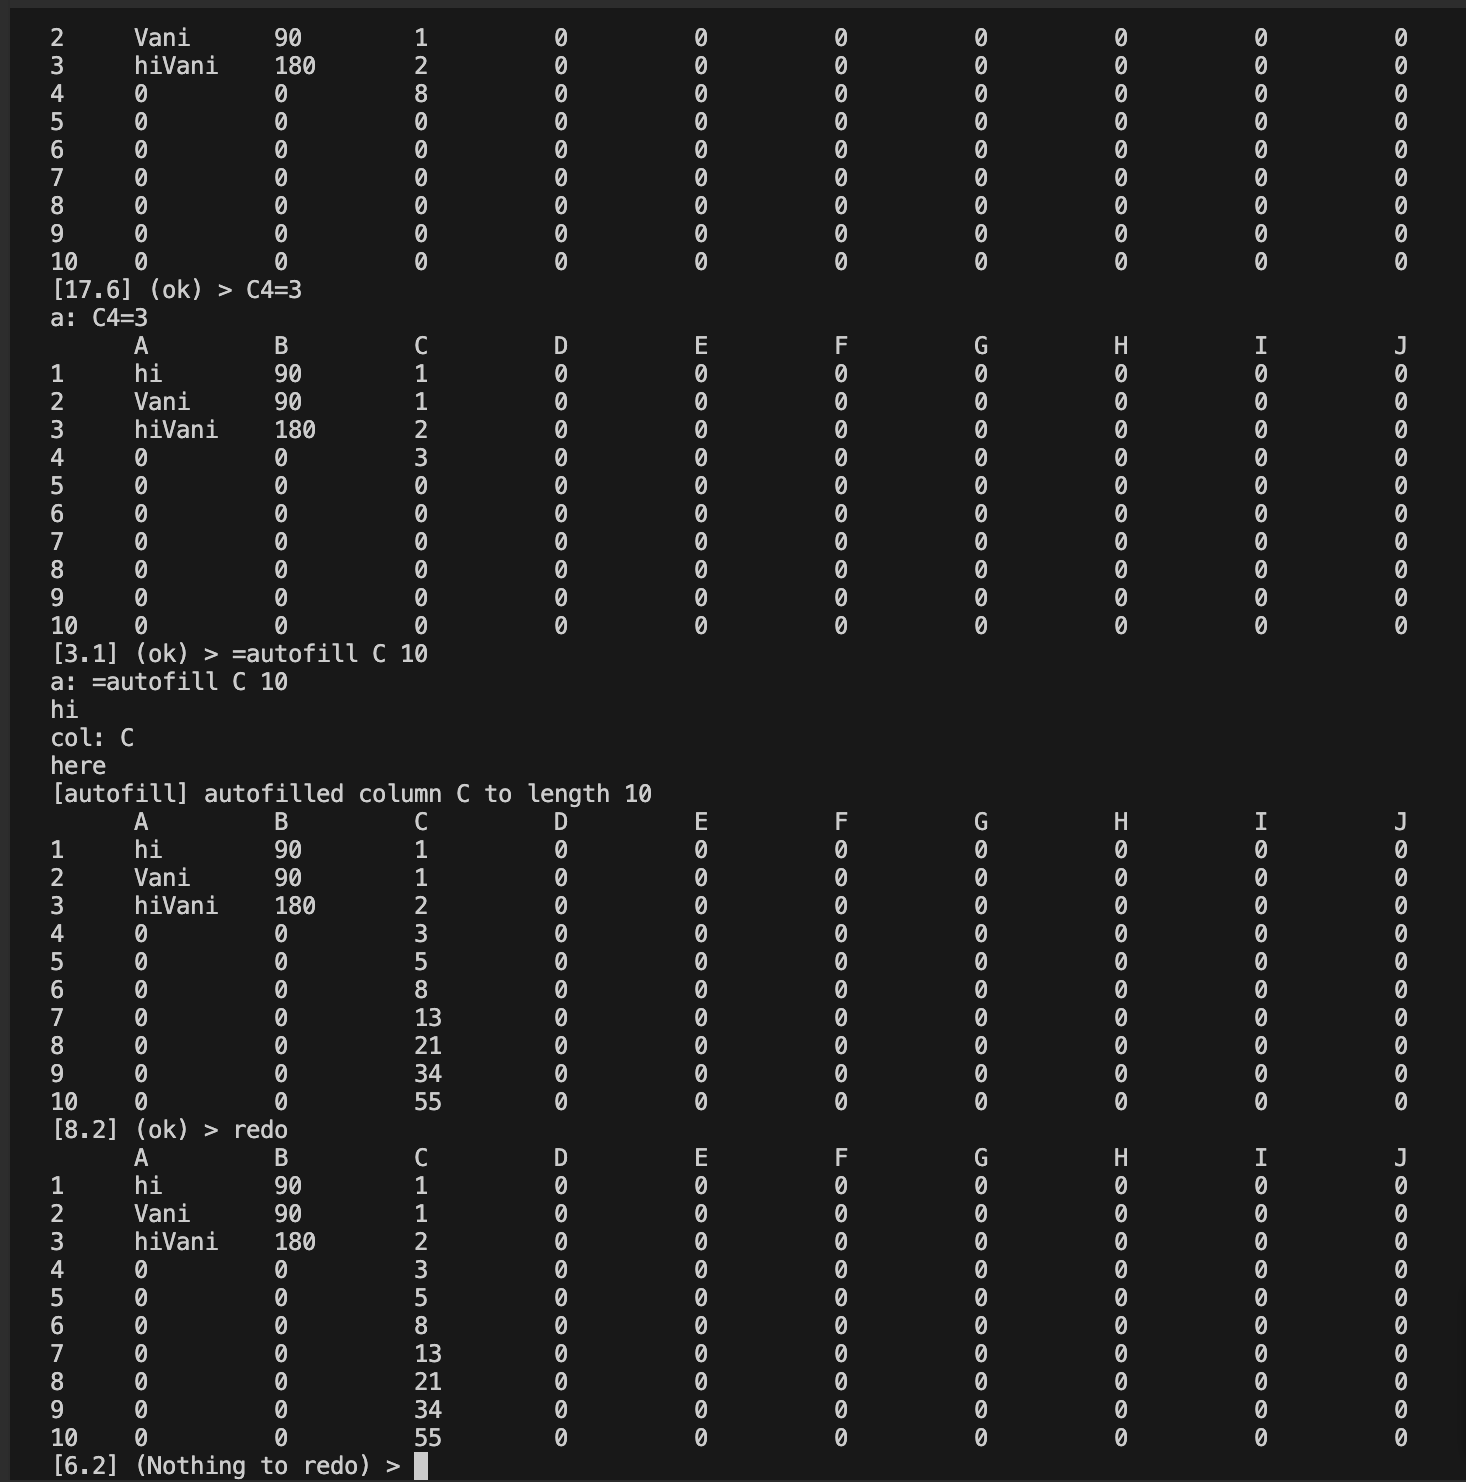
\includegraphics[width=0.5\linewidth]{image.png}
            \caption{Performing autofill for fibonacci}
            \label{fig:enter-label}
        \end{figure}
        
%----------------------------------------------------------

\printbibliography

\end{document}